En este capítulo se describen a alto nivel las funcionalidades principales que componen la versión final de la plataforma \textbf{Sky Apartments}, detallando la experiencia de usuario y las herramientas de gestión desarrolladas. 

Para facilitar la comprensión del sistema y ofrecer una visión dinámica de su funcionamiento, se ha elaborado un vídeo demostrativo alojado en YouTube, accesible a través del siguiente enlace:
\newline
\url{https://www.youtube.com/watch?v=wLvm_5JjNUs}.

Las funcionalidades detalladas se recogen en el Anexo~\ref{anexo:funcionalidades-detalladas}, y las instrucciones de instalación y ejecución en el Anexo~\ref{anexo:instrucciones-ejecutar-aplicacion}.
\section{Roles de Usuario}
El sistema ha sido diseñado bajo una arquitectura de control de acceso basada en roles (RBAC), distinguiendo tres niveles de interacción con la plataforma:
\begin{itemize}
    \item \textbf{Usuario Anónimo:} Puede navegar por el catálogo de apartamentos, utilizar los filtros de búsqueda, visualizar los detalles de los apartamentos y comprobar la disponibilidad en el calendario, pero no puede formalizar reservas.
    \item \textbf{Usuario Registrado:} Dispone de un área personal. Además de las acciones del usuario anónimo, puede realizar reservas, gestionar su historial, cancelar estancias activas y publicar reseñas tras finalizar su viaje.
    \item \textbf{Administrador:} Tiene acceso exclusivo al panel de control (\textit{Dashboard}). Desde allí gestiona el catálogo de apartamentos (CRUD), supervisa todas las reservas del sistema y visualiza las estadísticas de negocio.
\end{itemize}

\section{Navegación y Búsqueda de Alojamientos}
Esta sección describe el sistema de filtrado avanzado para explorar el catálogo de alojamientos según criterios personalizados, y la página de detalle de cada apartamento, que centraliza la galería multimedia y el calendario interactivo con precios dinámicos.
\subsection{Catálogo y Filtrado Avanzado}
Las páginas de visualización de apartamentos ofrecen un catálogo interactivo de apartamentos presentados mediante un diseño de tarjetas (\textit{cards}) (ver Figuras \ref{fig:advanced_filters} y \ref{fig:catalogo_apartamentos}). Para facilitar la búsqueda, se ha implementado un motor de filtrado avanzado que permite a los usuarios combinar múltiples criterios:
\begin{itemize}
    \item \textbf{Capacidad:} Filtrado por número de huéspedes.
    \item \textbf{Comodidades:} Selección de características específicas (terraza, balcón, aparcamiento, piscina, etc.).
    \item \textbf{Disponibilidad:} Búsqueda por rango de fechas exactas.
    \item \textbf{Valoración mínima:} Filtrado basado en la puntuación otorgada por huéspedes anteriores (1 a 5 estrellas).
\end{itemize}

\begin{figure}[!h]
    \centering
    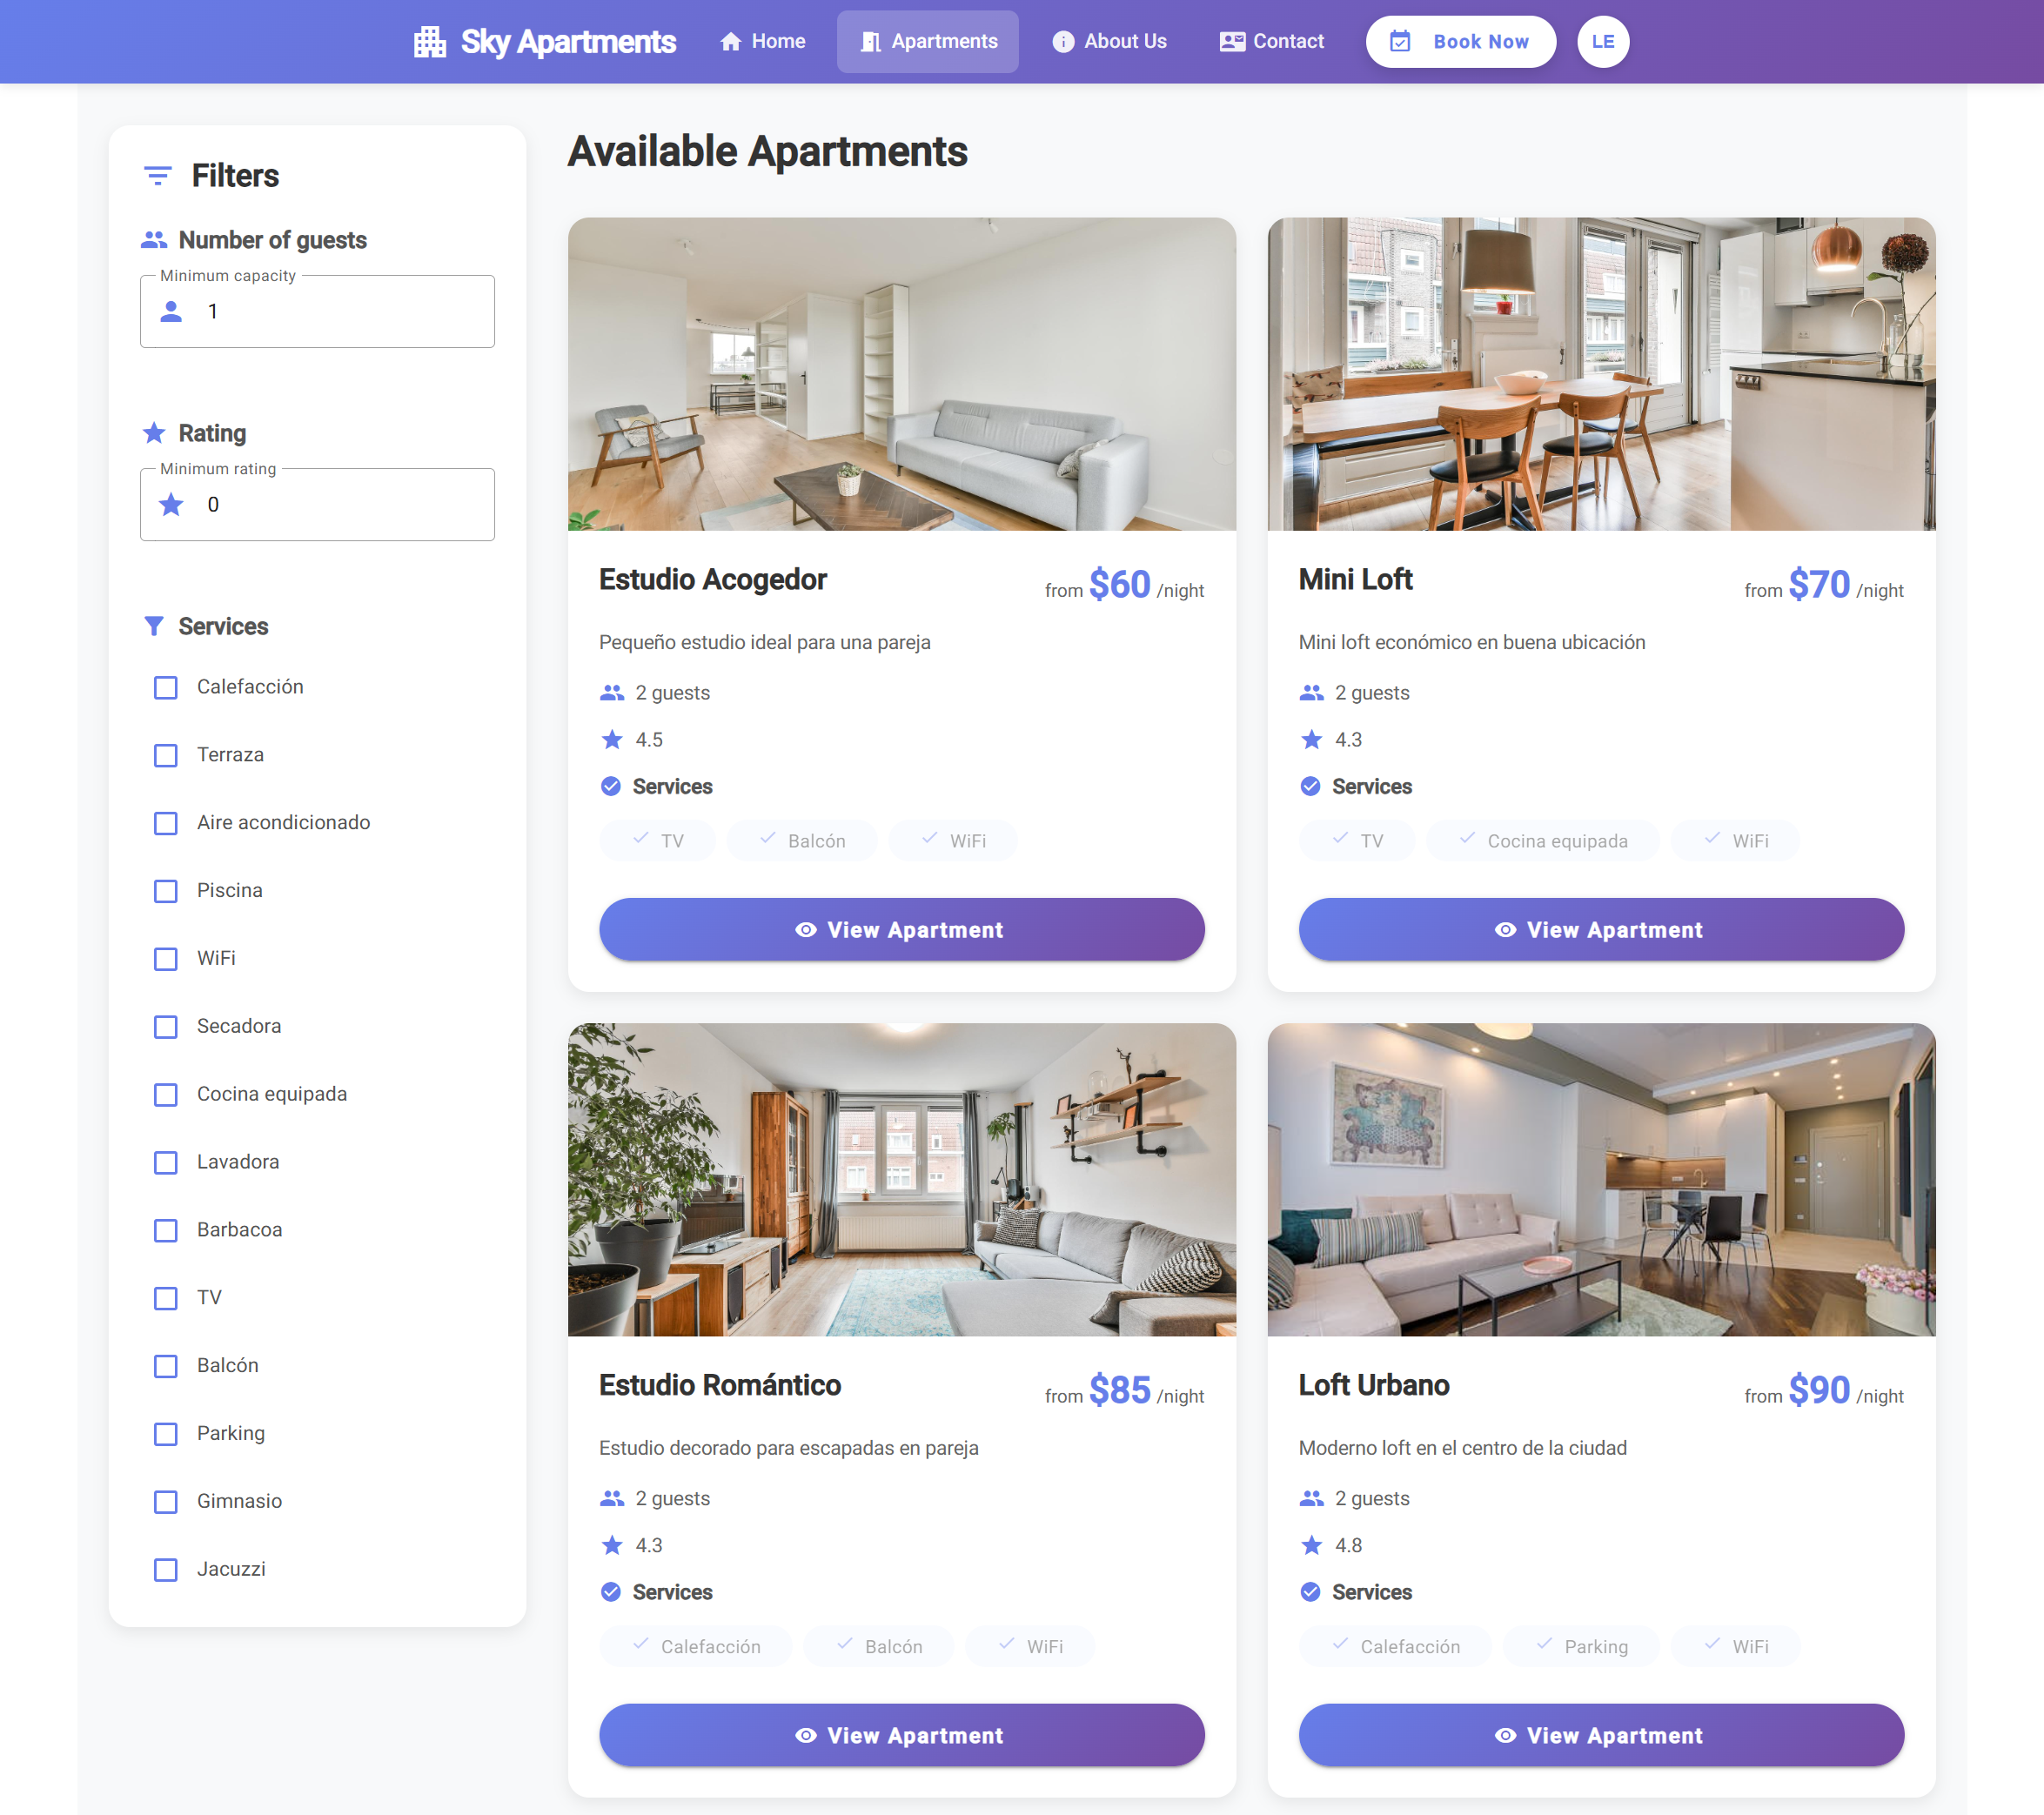
\includegraphics[width=0.8\textwidth]{img/advanced_filters_v1.png}
    \caption{Interfaz del motor de búsqueda con filtros avanzados combinados.}
    \label{fig:advanced_filters}
\end{figure}

\begin{figure}[!h]
    \centering
    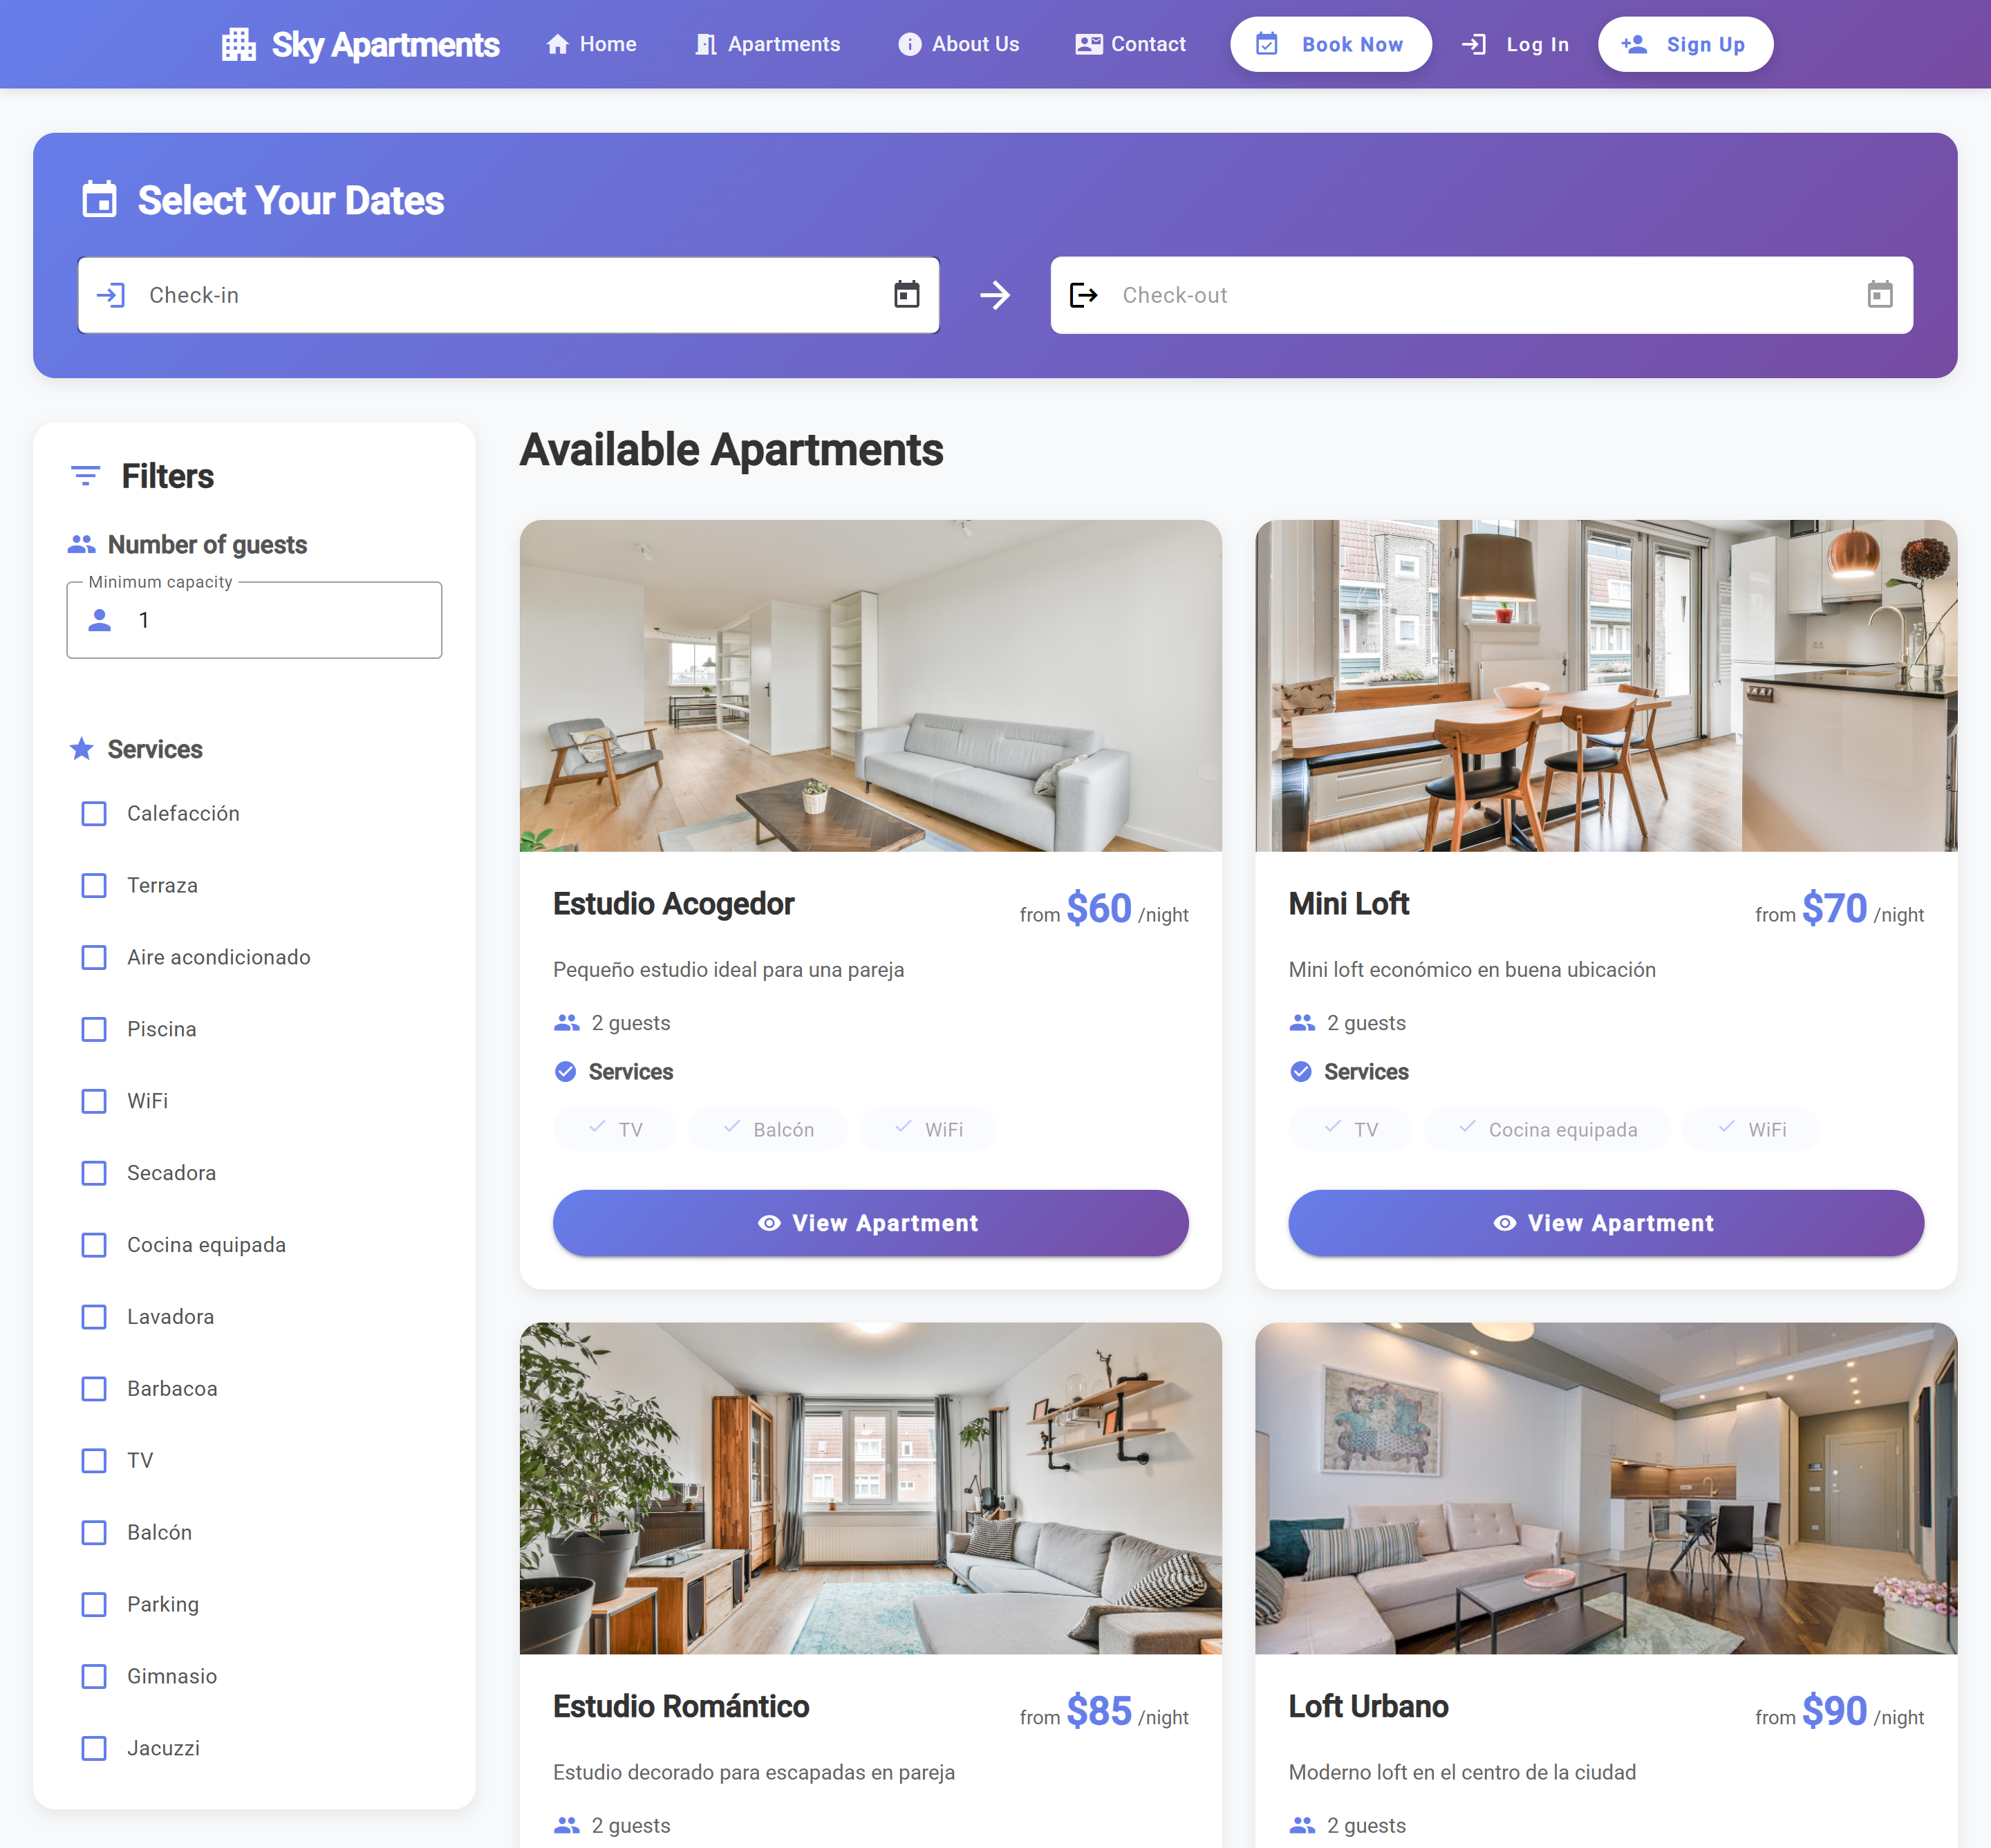
\includegraphics[width=0.8\textwidth]{img/catalogo_apartamentos_2.png}
    \caption{Interfaz del catálogo de apartamentos con filtro por fecha.}
    \label{fig:catalogo_apartamentos}
\end{figure}

\subsection{Detalles del Apartamento e Interfaz de Precios}
Cada alojamiento dispone de una página de detalle exhaustiva. En ella, el usuario puede interactuar con una galería multimedia de alta calidad,  consultar la descripción completa y los servicios incluidos (ver Figura \ref{fig:apartment_detail}).

Uno de los aspectos más destacados de esta vista es el \textbf{calendario interactivo con precios dinámicos}. El sistema no muestra una tarifa plana, sino que calcula y muestra variaciones de precio basadas en la temporada (alta, media, baja), el día de la semana (fines de semana), la proximidad de la fecha de reserva (\textit{last-minute}) o cualquier ajuste del precio que configure el administrador. Esto ofrece total transparencia al usuario, mostrando el desglose entre el precio base y las modificaciones aplicadas.

\begin{figure}[!h]
    \centering
    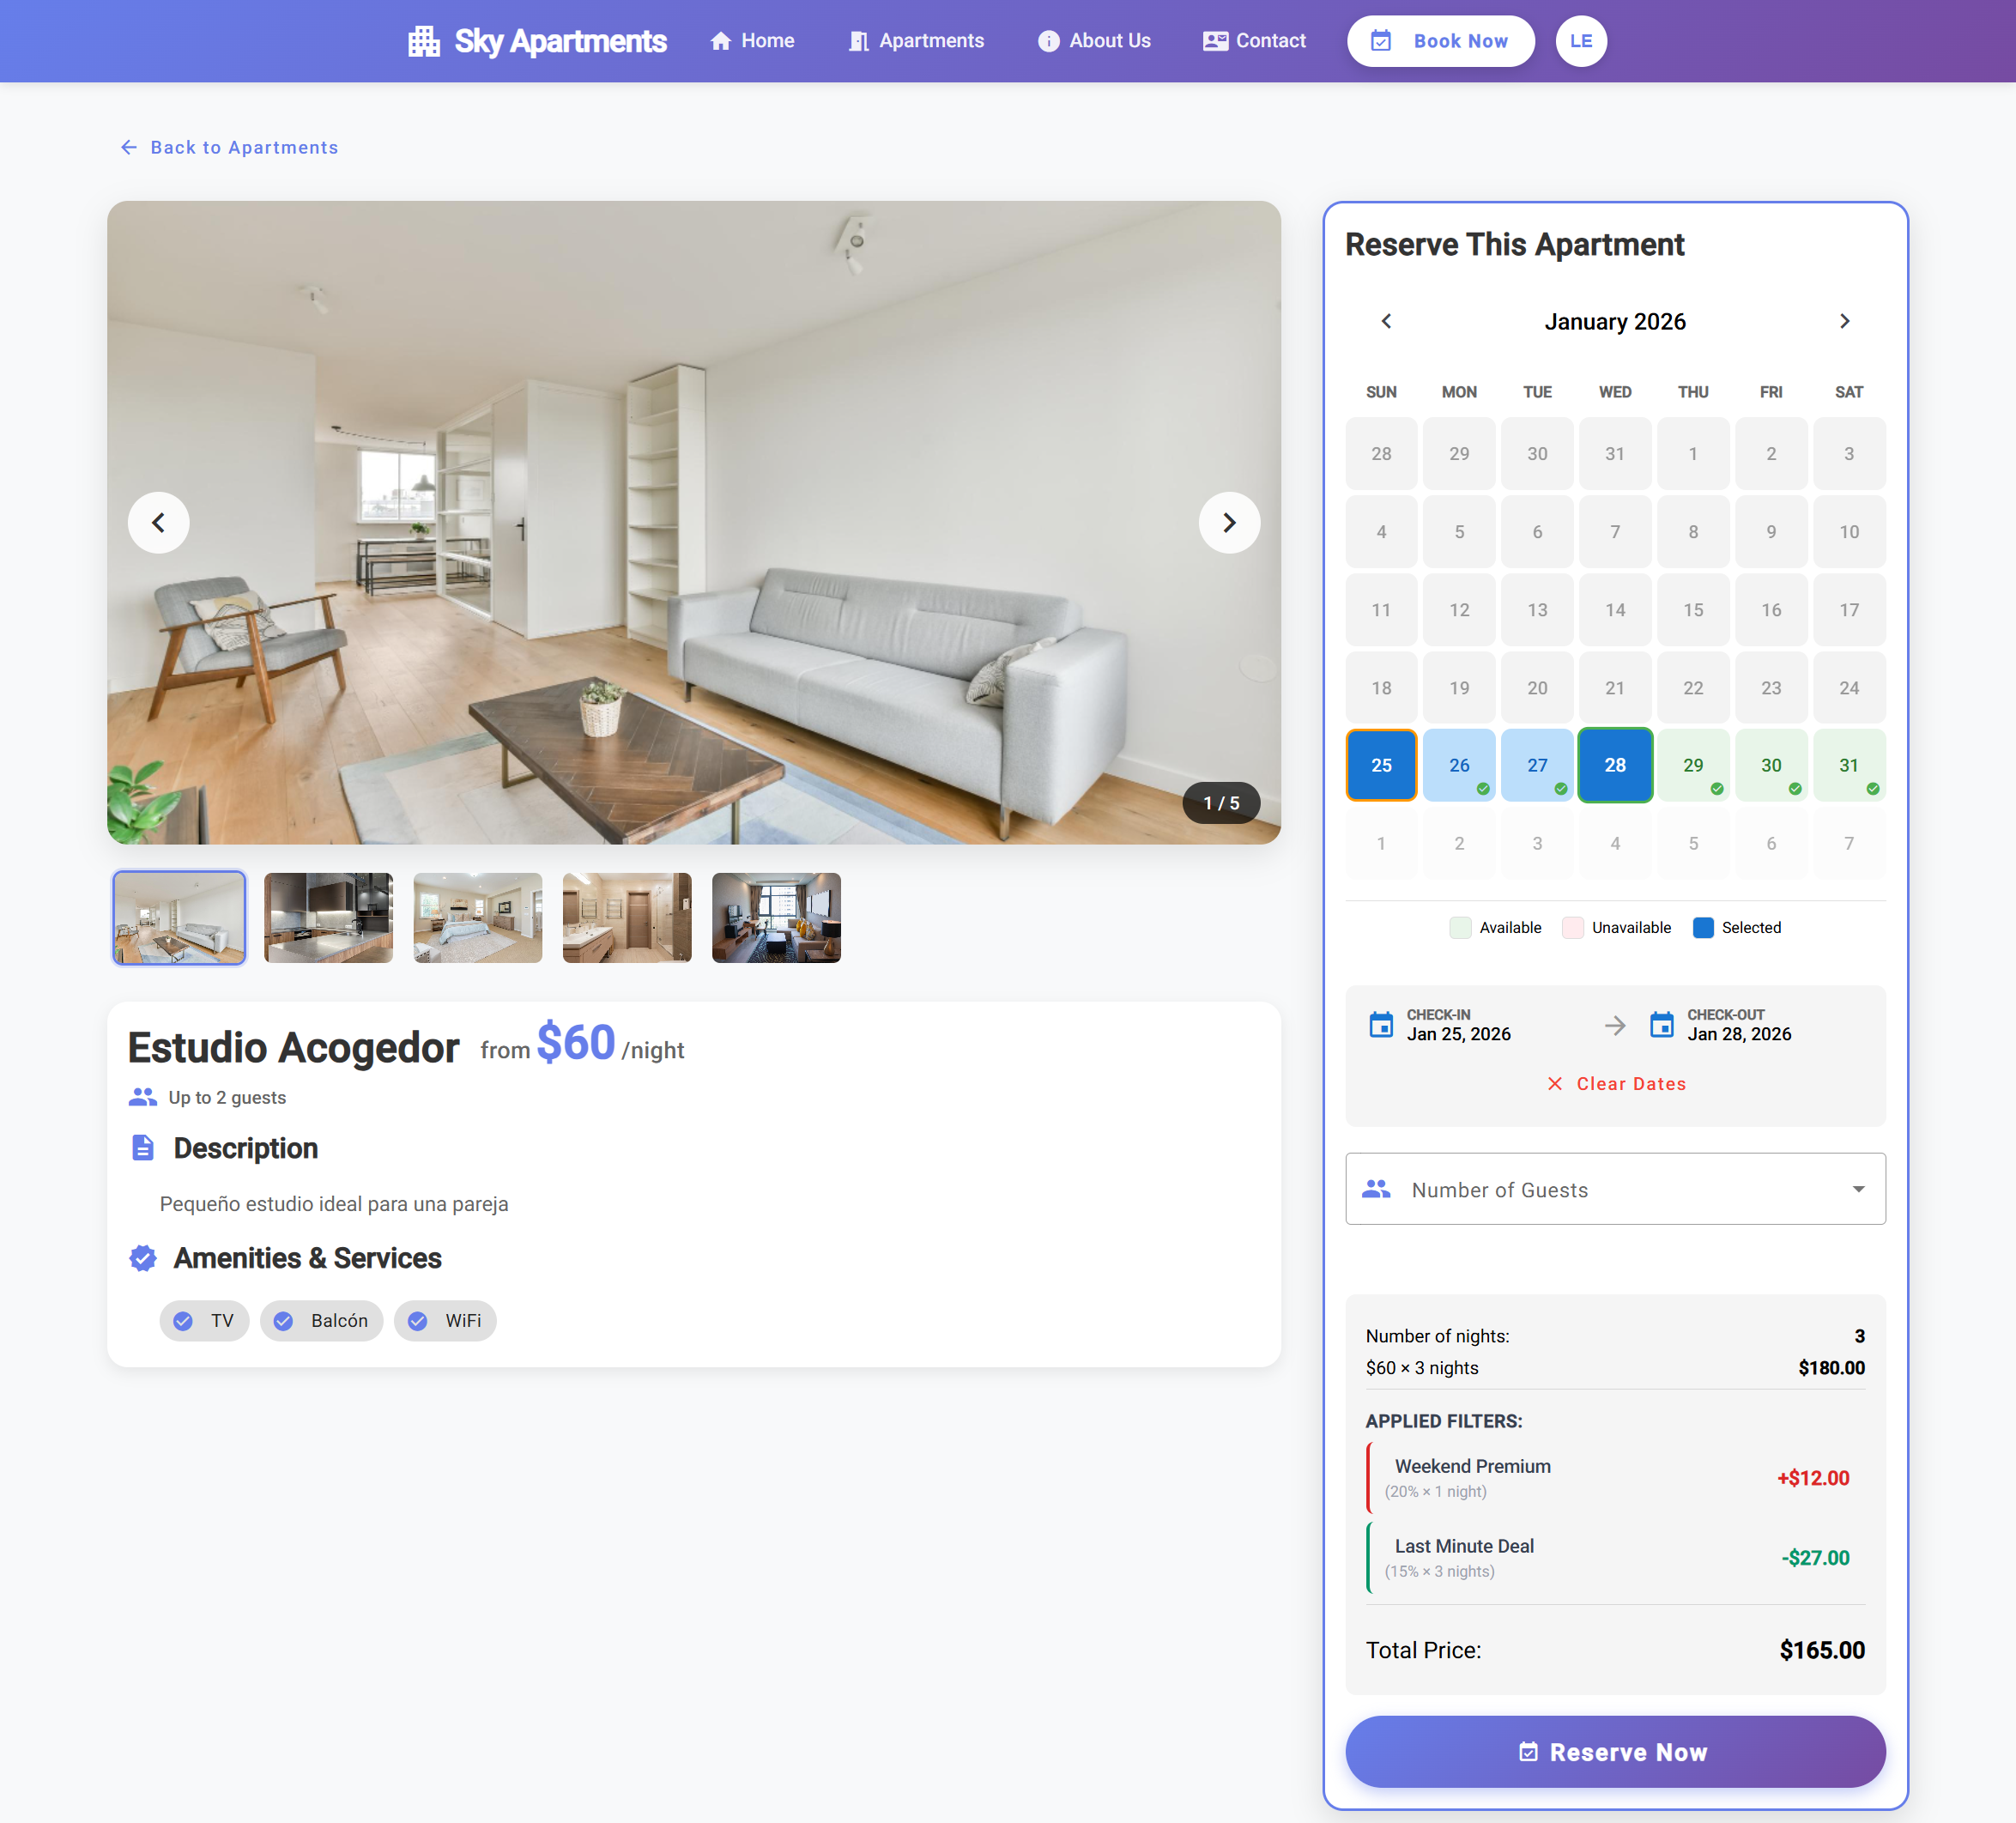
\includegraphics[width=1\textwidth]{img/apartment_detail_v1.png}
    \caption{Página de detalle del apartamento mostrando la galería multimedia y el calendario dinámico con precios.}
    \label{fig:apartment_detail}
\end{figure}

\section{Gestión del Ciclo de Vida de la Reserva}

El proceso de reserva ha sido diseñado para ser intuitivo y seguro. Una vez que el usuario registrado selecciona las fechas y el número de huéspedes, el sistema presenta un resumen detallado con el desglose final del precio.

\subsection{Sincronización y Notificaciones}
Al confirmar una reserva, el sistema ejecuta dos acciones críticas de forma simultánea:
\begin{enumerate}
    \item \textbf{Sincronización inmediata:} Actualiza el calendario global de disponibilidad en tiempo real, bloqueando las fechas para evitar cualquier posibilidad de \textit{overbooking}.
    \item \textbf{Notificaciones transaccionales automáticas:} El usuario recibe correos electrónicos automáticos en cada etapa de la reserva: confirmaciones, actualizaciones, cancelaciones y recordatorios de \textit{check-in} (ver Figura~\ref{fig:booking_confirmation}).
\end{enumerate}

\begin{figure}[!h]
    \centering
    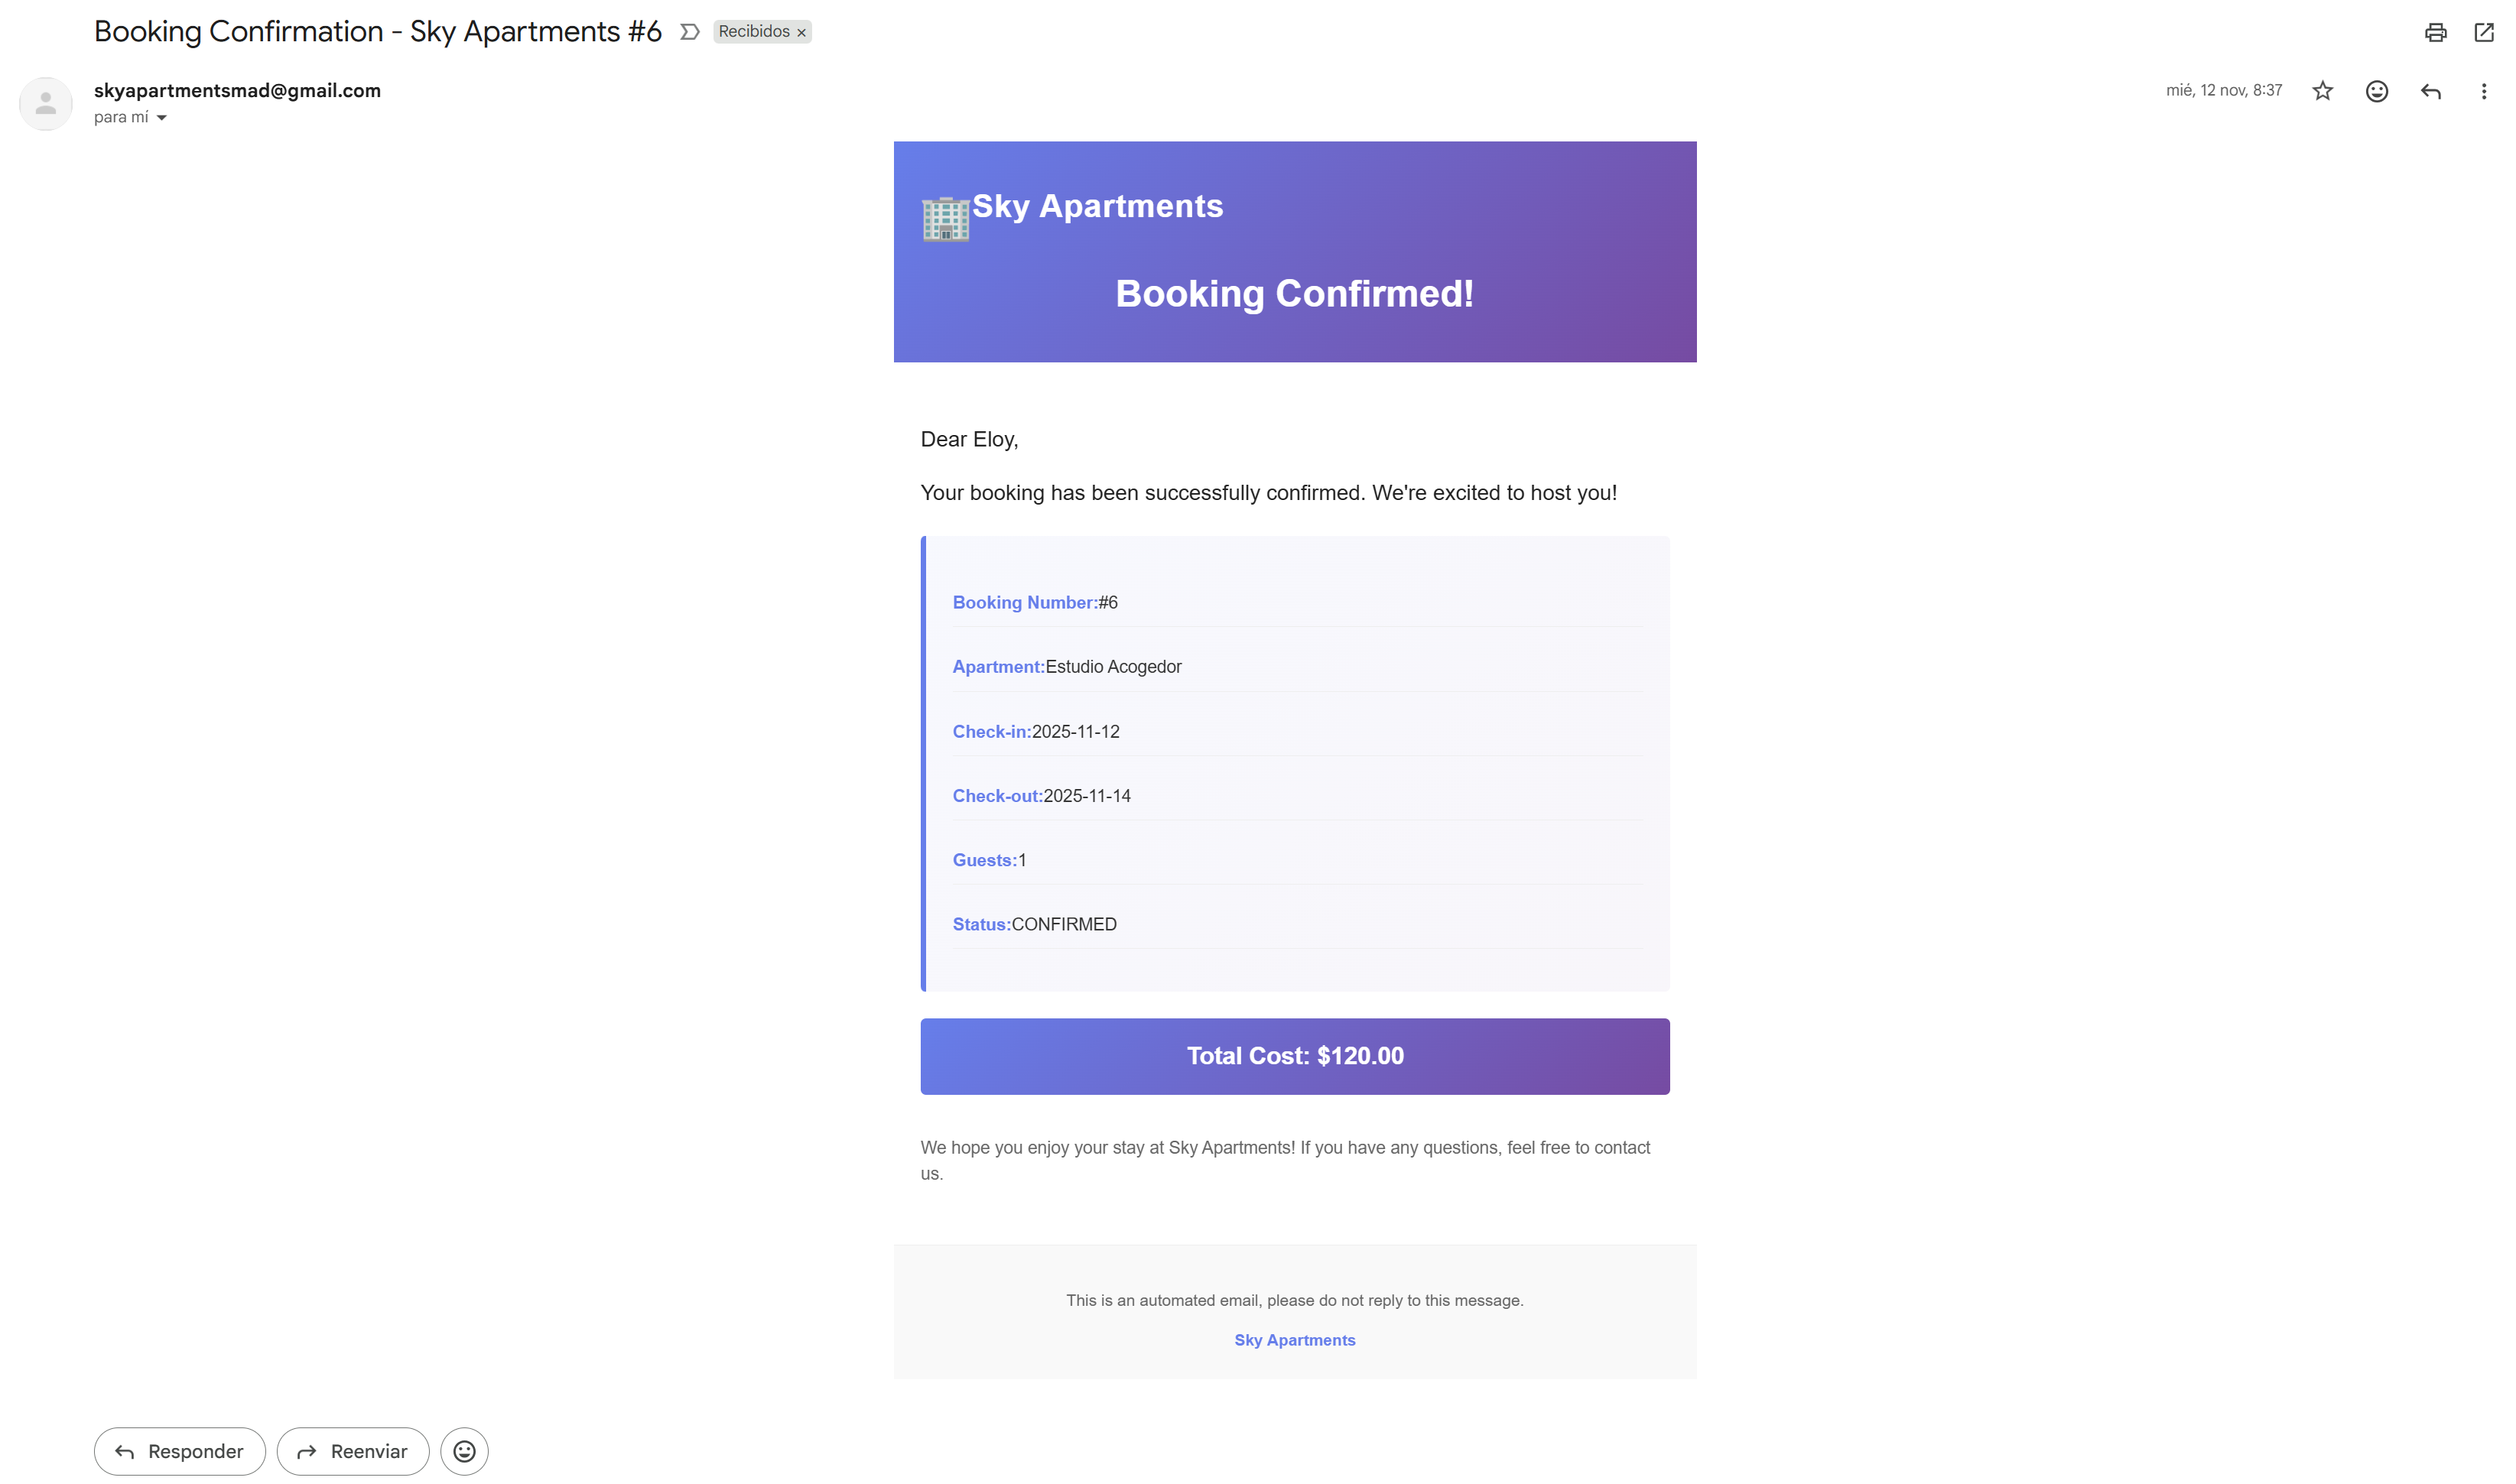
\includegraphics[width=1\textwidth]{img/booking_confirmation_v02.png}
    \caption{Ejemplo de notificación de confirmación de reserva enviada al usuario.}
    \label{fig:booking_confirmation}
\end{figure}

\section{Área de Usuario y Sistema de Reseñas}
Esta sección describe el panel personal del usuario registrado, desde el que puede gestionar su perfil e historial de estancias, y el sistema de reseñas para valorar los alojamientos tras su visita.
\subsection{Perfil e Historial}
Los usuarios registrados disponen de un panel personal donde pueden actualizar sus datos y consultar su historial completo de reservas. Este panel categoriza las reservas por estado (confirmadas, canceladas o completadas) y permite la cancelación ágil de estancias futuras.

\subsection{Valoraciones y Prueba Social}
Para fomentar la confianza en la plataforma, se ha implementado un sistema de reseñas. Una vez que el estado de una reserva pasa a "completada" (tras el \textit{check-out}), el usuario queda habilitado para puntuar el alojamiento (1-5 estrellas) y redactar un comentario detallado sobre su experiencia. Estas reseñas se publican en la página del apartamento, alimentando el algoritmo de valoración media (ver Figura \ref{fig:reviews}).

\begin{figure}[!h]
    \centering
    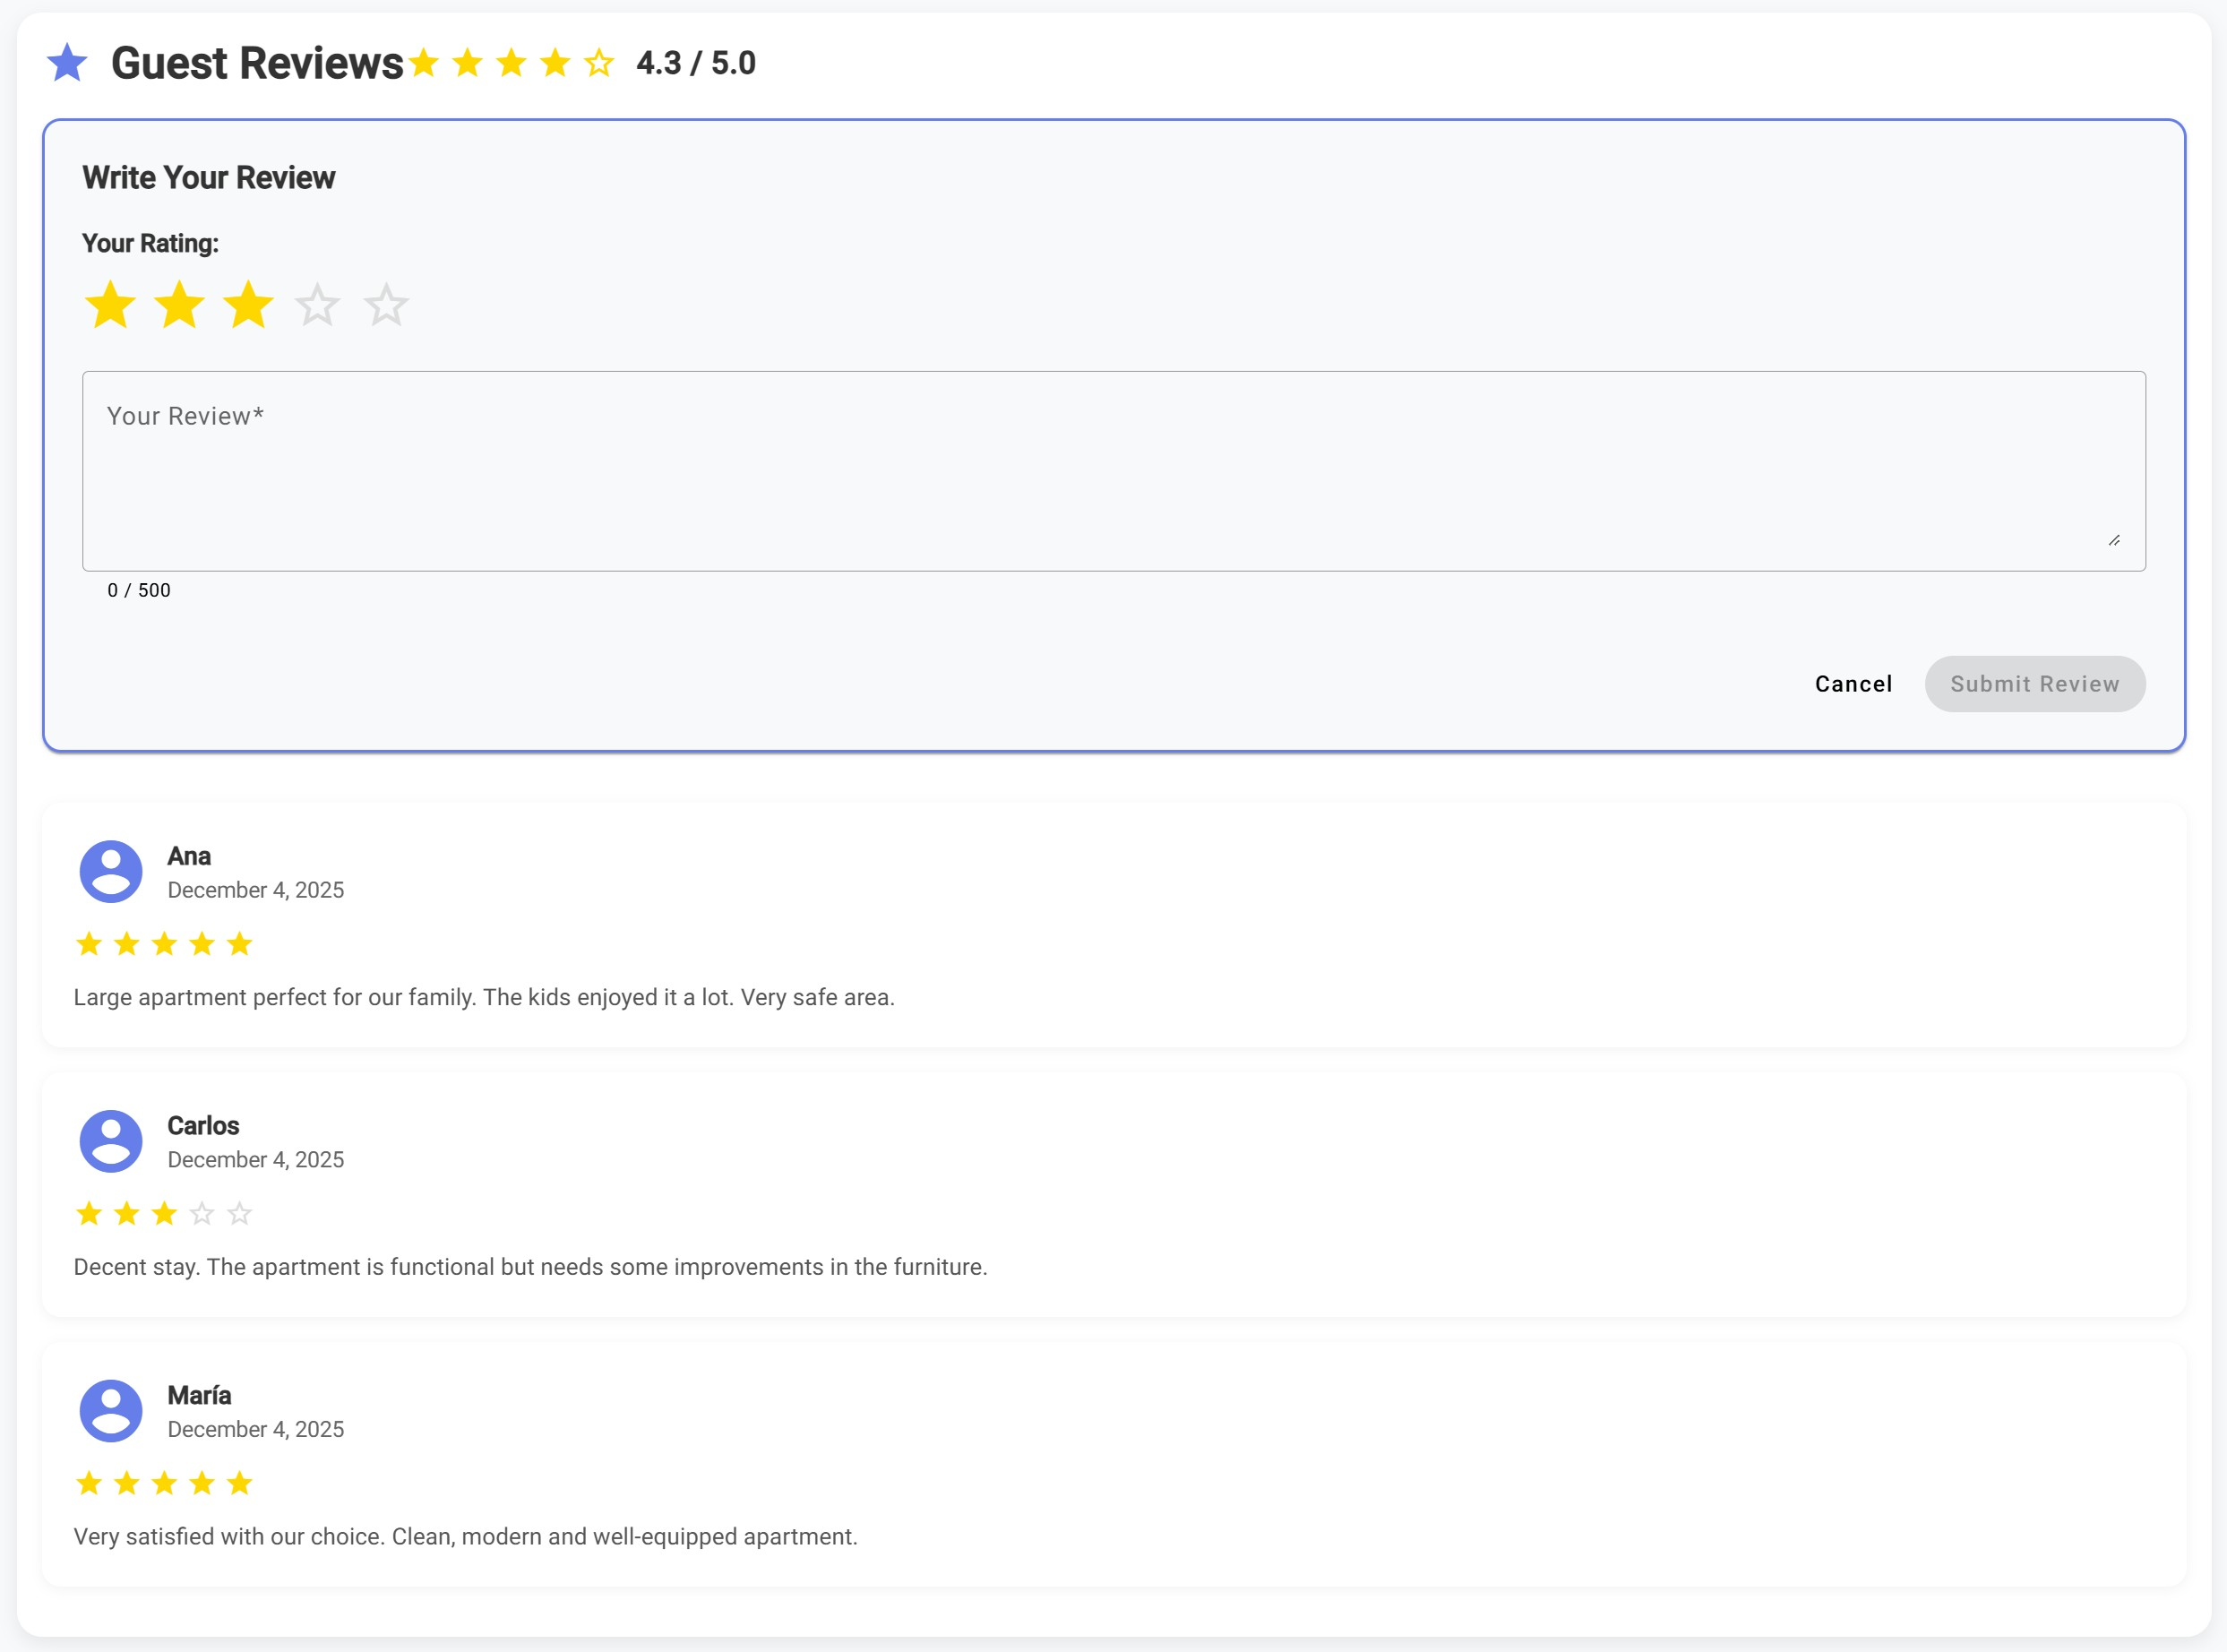
\includegraphics[width=0.9\textwidth]{img/reviews_v02.jpg}
    \caption{Sistema de valoraciones y reseñas integrado en la plataforma.}
    \label{fig:reviews}
\end{figure}

\section{Panel de Administración (Dashboard)}

El panel de administración dota al propietario de un control absoluto sobre su negocio a través de cuatro módulos principales.

\subsection{Analítica y Estadísticas}
El sistema genera representaciones visuales e indicadores clave de rendimiento (\textit{Key Performance Indicators}, KPIs) 
en tiempo real para el período seleccionado, incluyendo ingresos totales, número de 
reservas activas, tasas de ocupación media, duración promedio de las estancias, rankings 
de alojamientos más demandados y mejor valorados, y un gráfico de evolución temporal de 
ocupación (ver Figura~\ref{fig:admin_dashboard}).

\begin{figure}[!h]
    \centering
    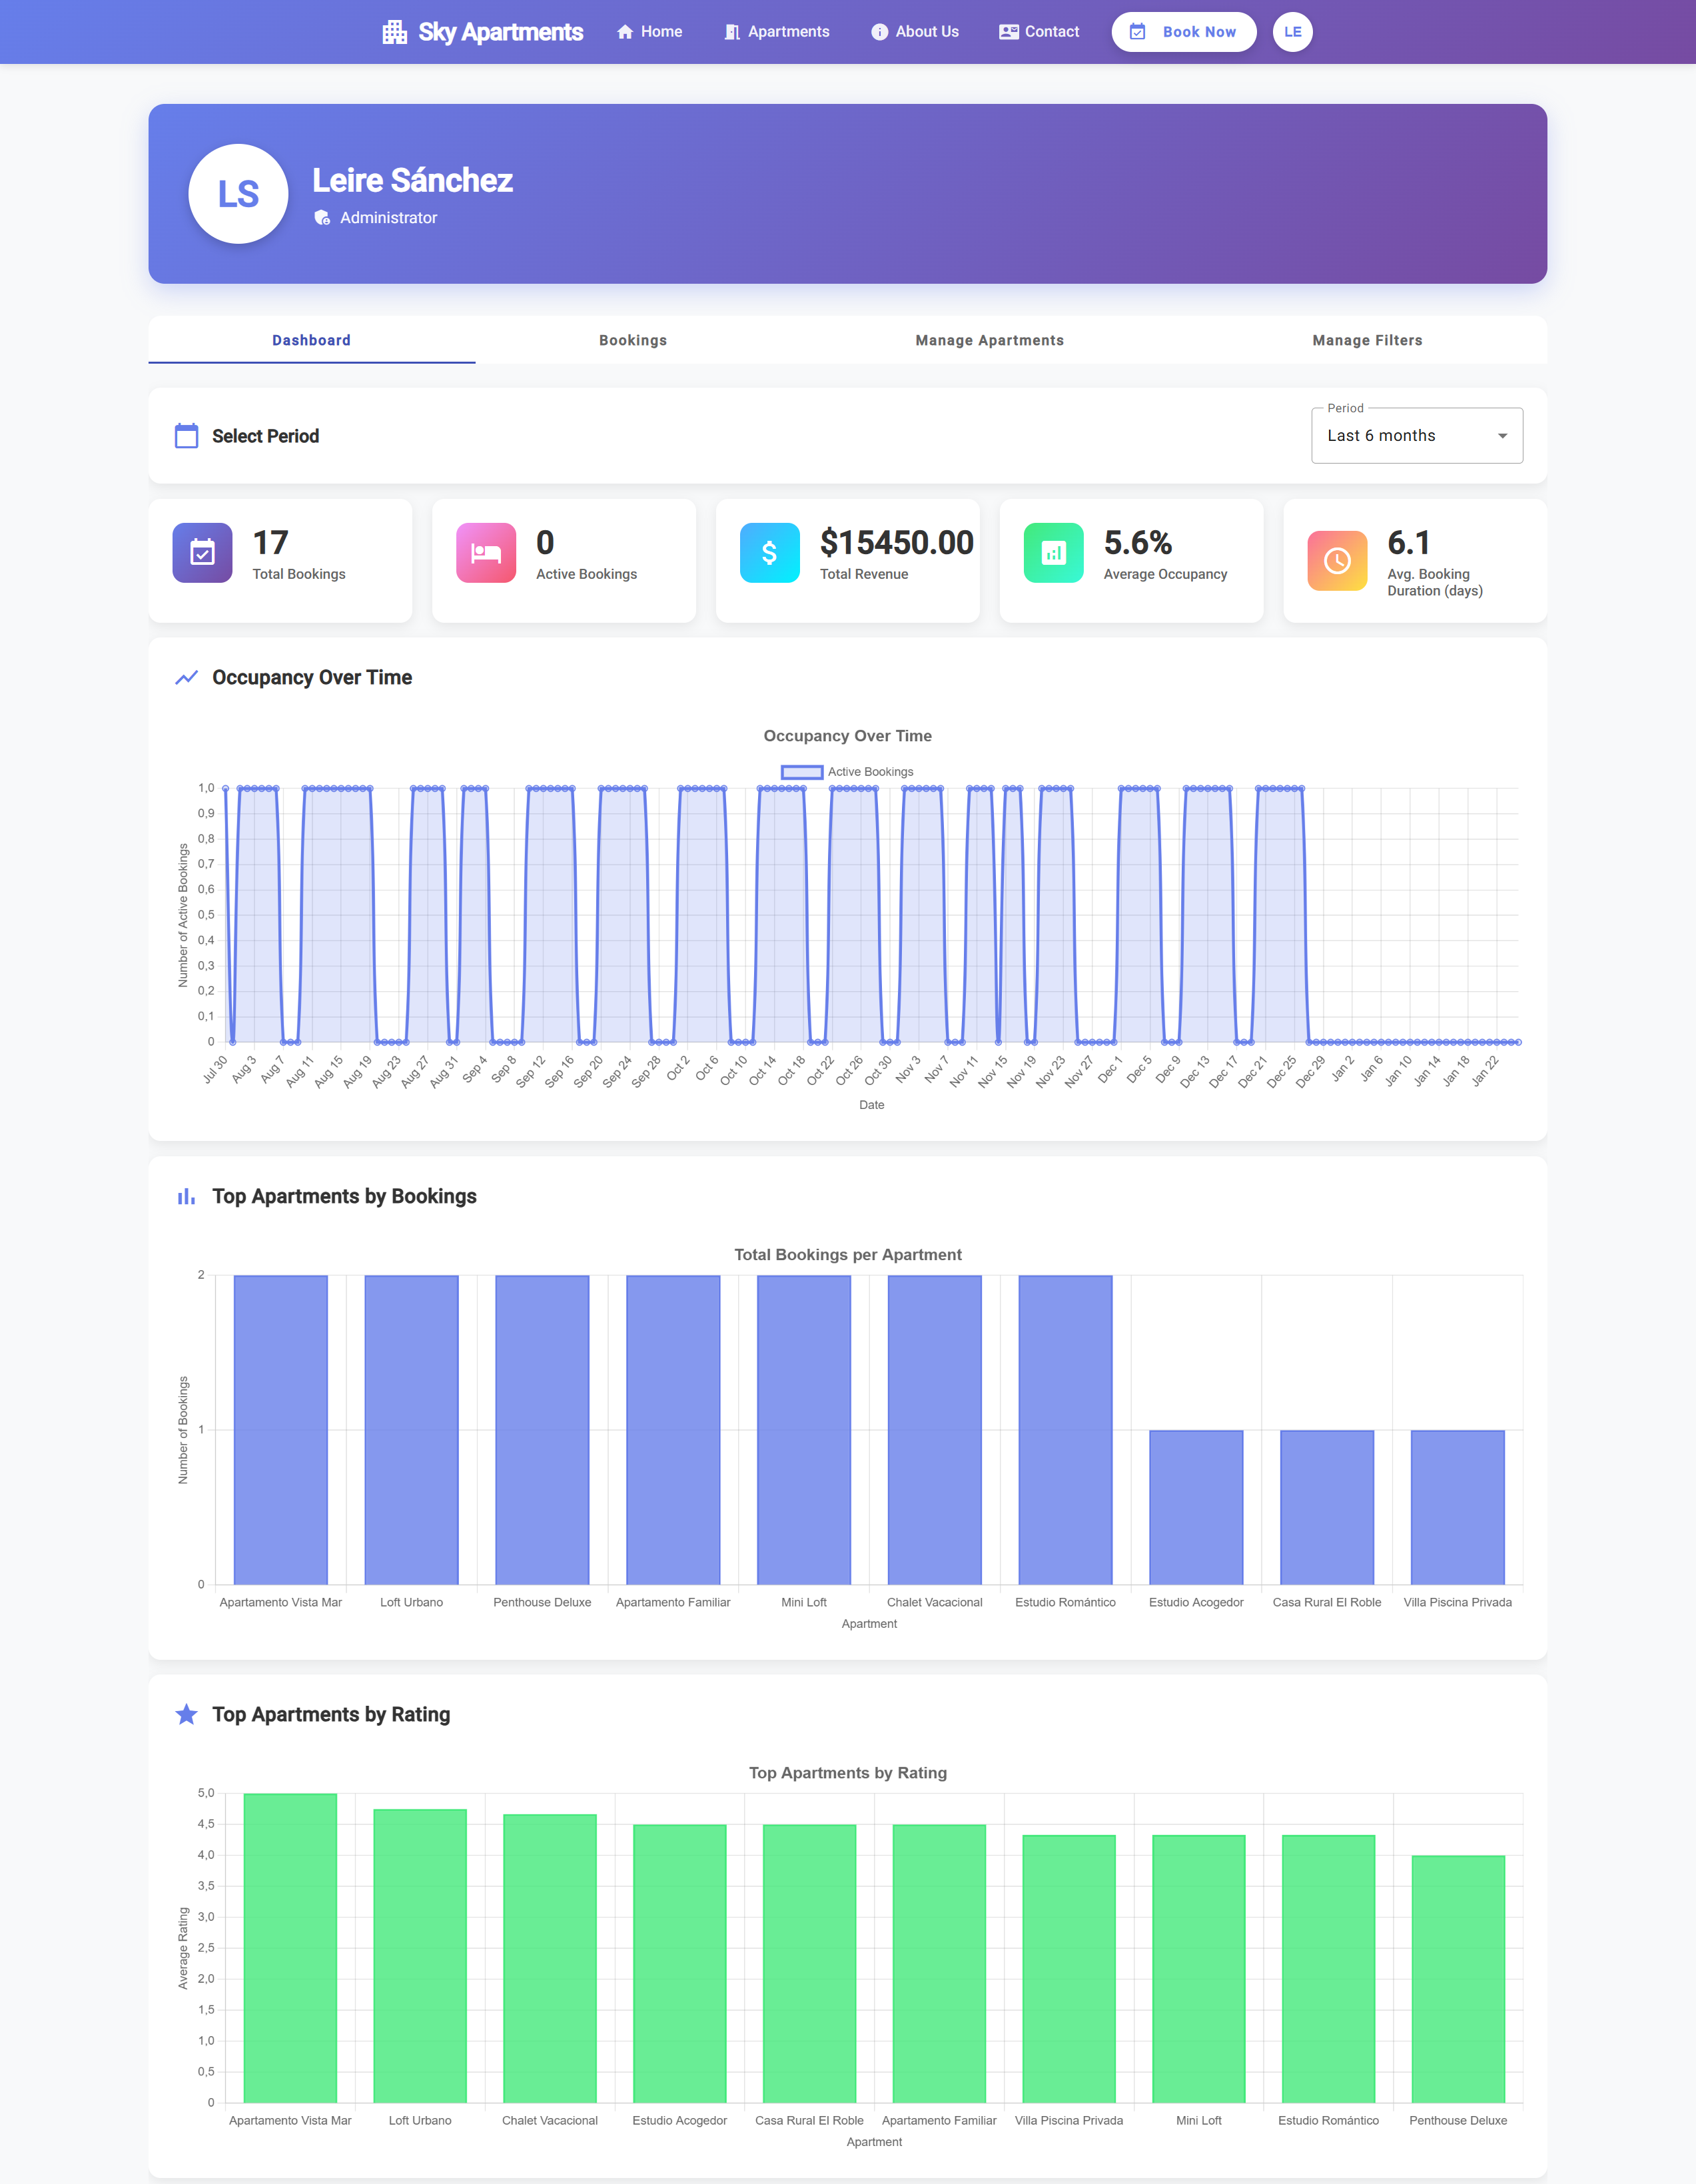
\includegraphics[width=0.9\textwidth]{img/admin_panel_v1.png}
    \caption{Dashboard analítico del panel de administración.}
    \label{fig:admin_dashboard}
\end{figure}

\subsection{Gestión de Apartamentos (CRUD)}
Desde este módulo, el administrador puede dar de alta, editar y eliminar apartamentos, gestionar sus galerías de imágenes y configurar sus características técnicas (capacidad, servicios incluidos, precio base) (ver Figura~\ref{fig:admin_apartments}).
\begin{figure}[!h]
    \centering
    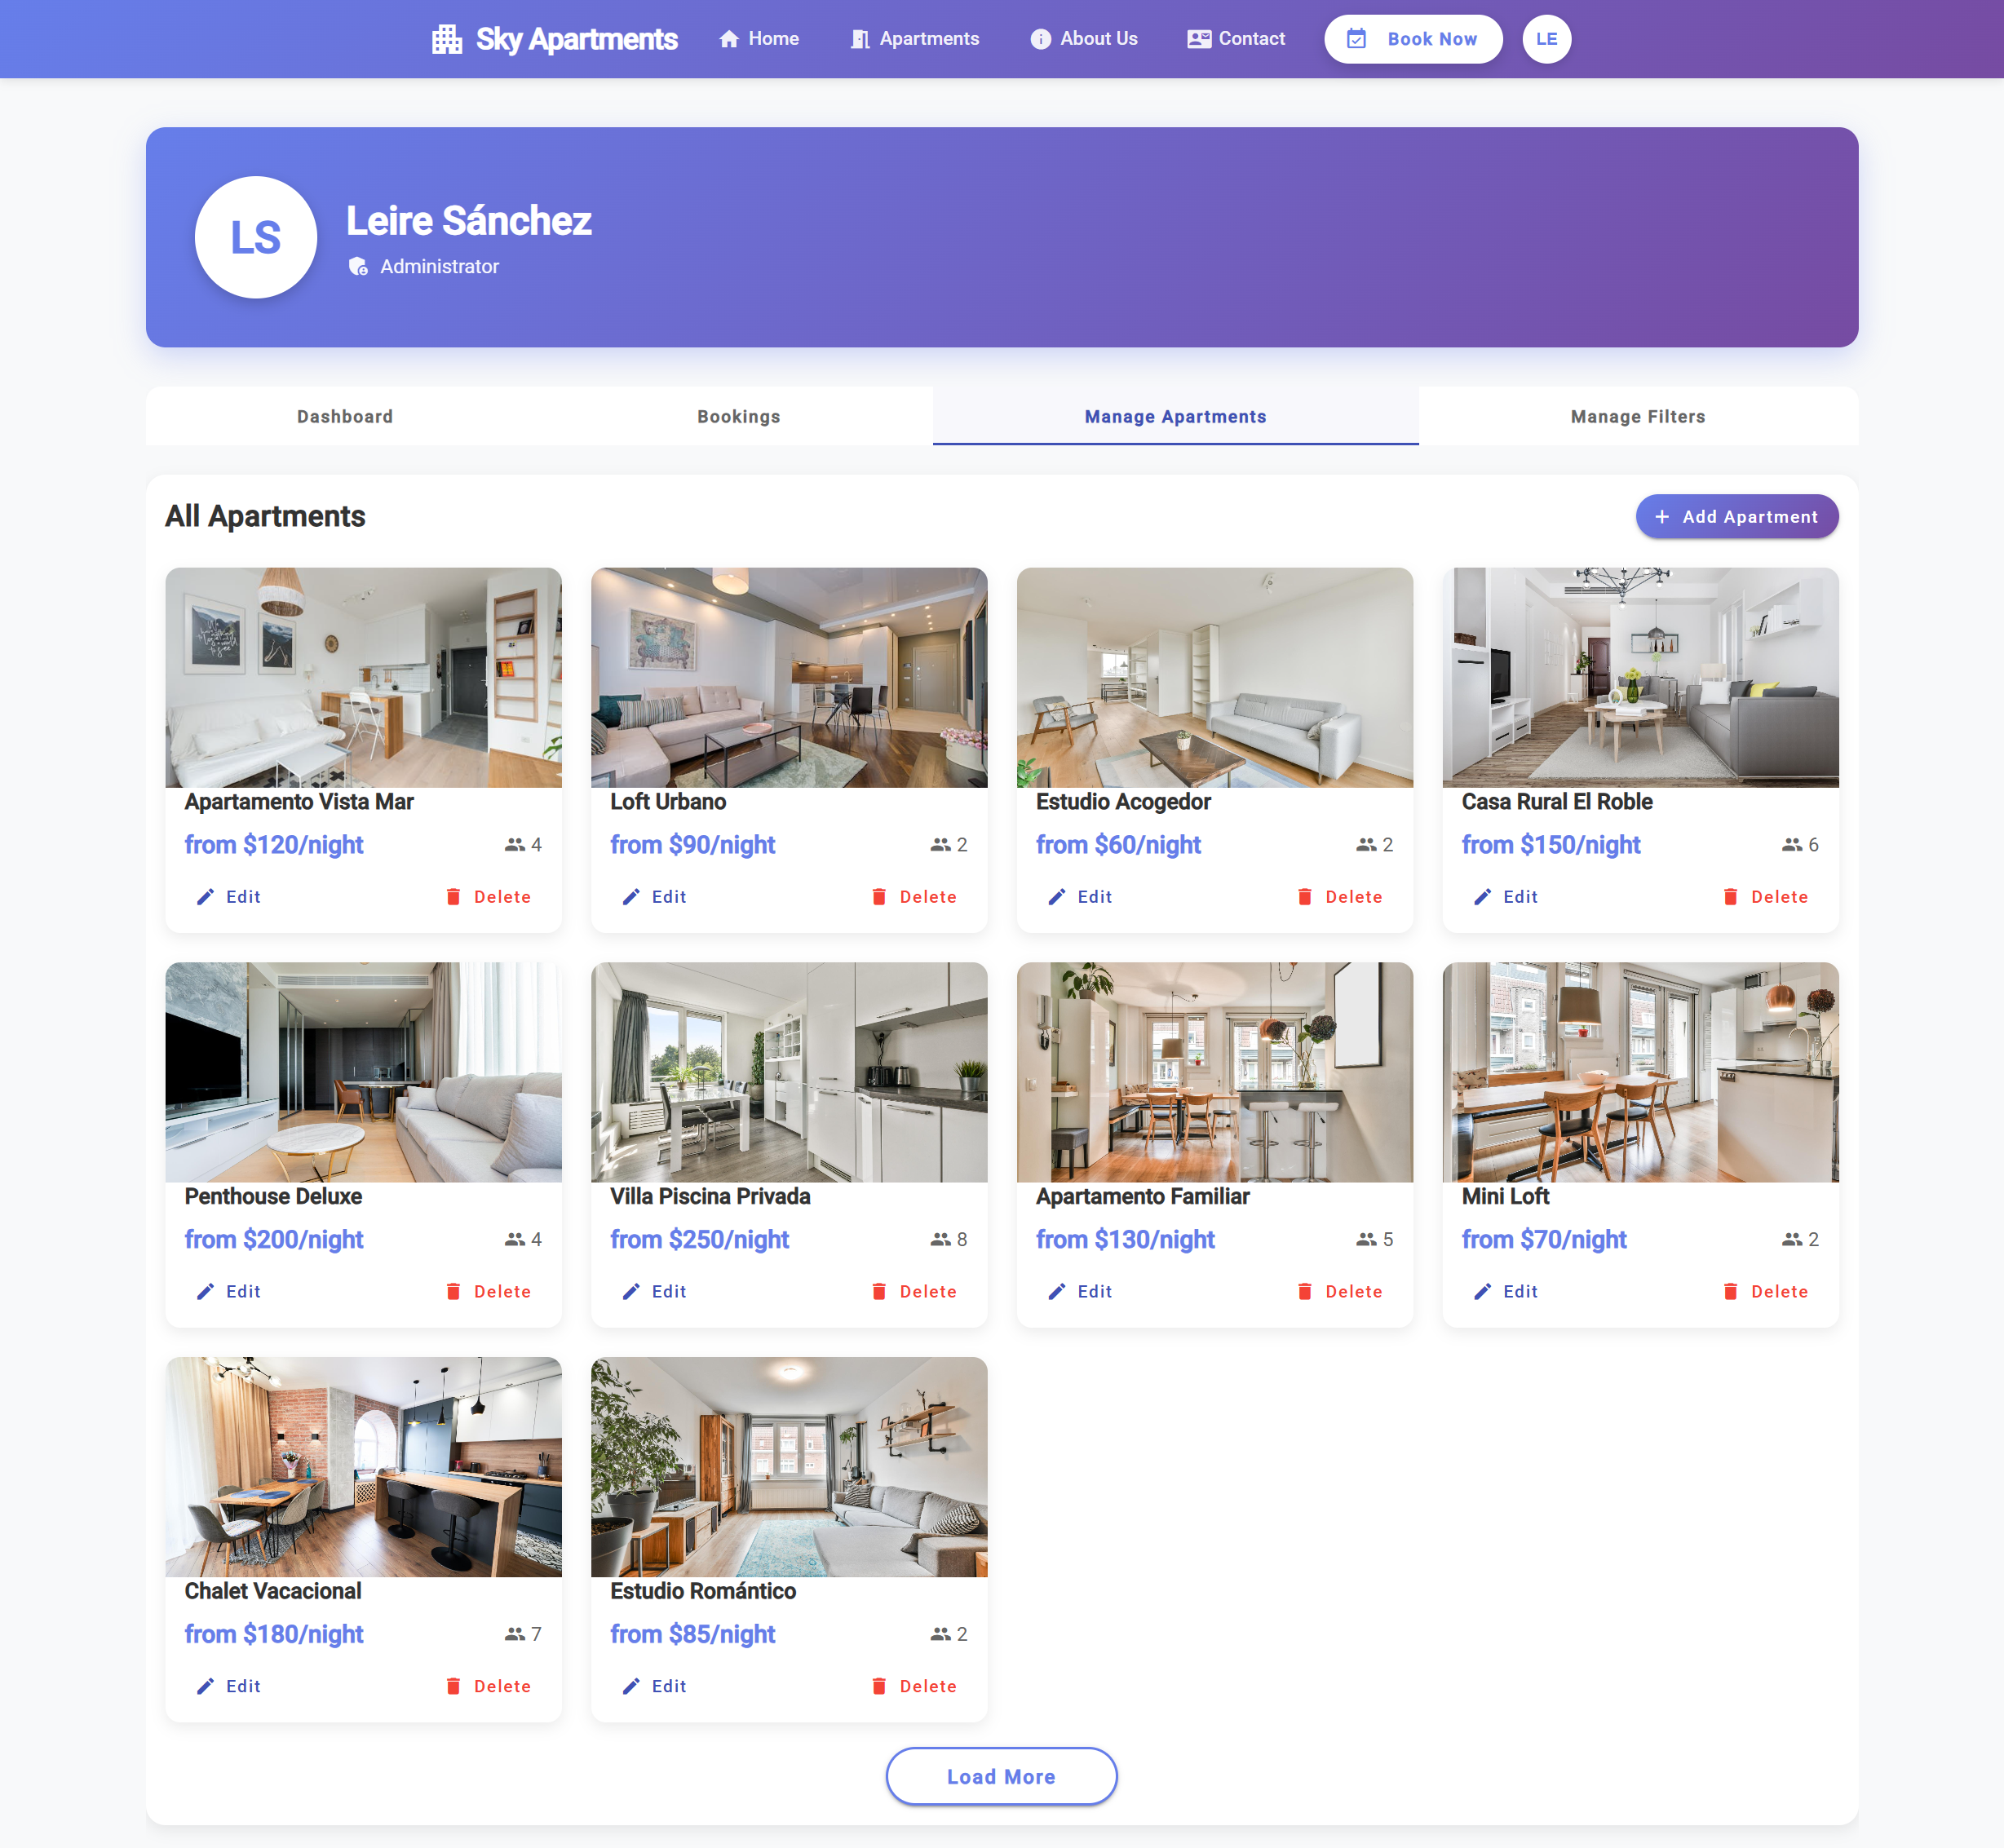
\includegraphics[width=0.9\textwidth]{img/admin_apartments_v1.png}
    \caption{Interfaz de gestión y edición del catálogo de apartamentos.}
    \label{fig:admin_apartments}
\end{figure}

\subsection{Gestión de Precios Dinámicos}
A nivel de negocio, este módulo independiente permite al administrador configurar las reglas del motor de precios dinámicos de forma visual. Desde aquí se pueden crear, activar o desactivar filtros de precio complejos: estableciendo multiplicadores de fin de semana, definiendo las fechas exactas de las distintas temporadas (alta, baja) y configurando ajustes automáticos por reservas de última hora (\textit{last minute}) o largas estancias (ver Figura \ref{fig:admin_filters}).

\begin{figure}[!h]
    \centering
    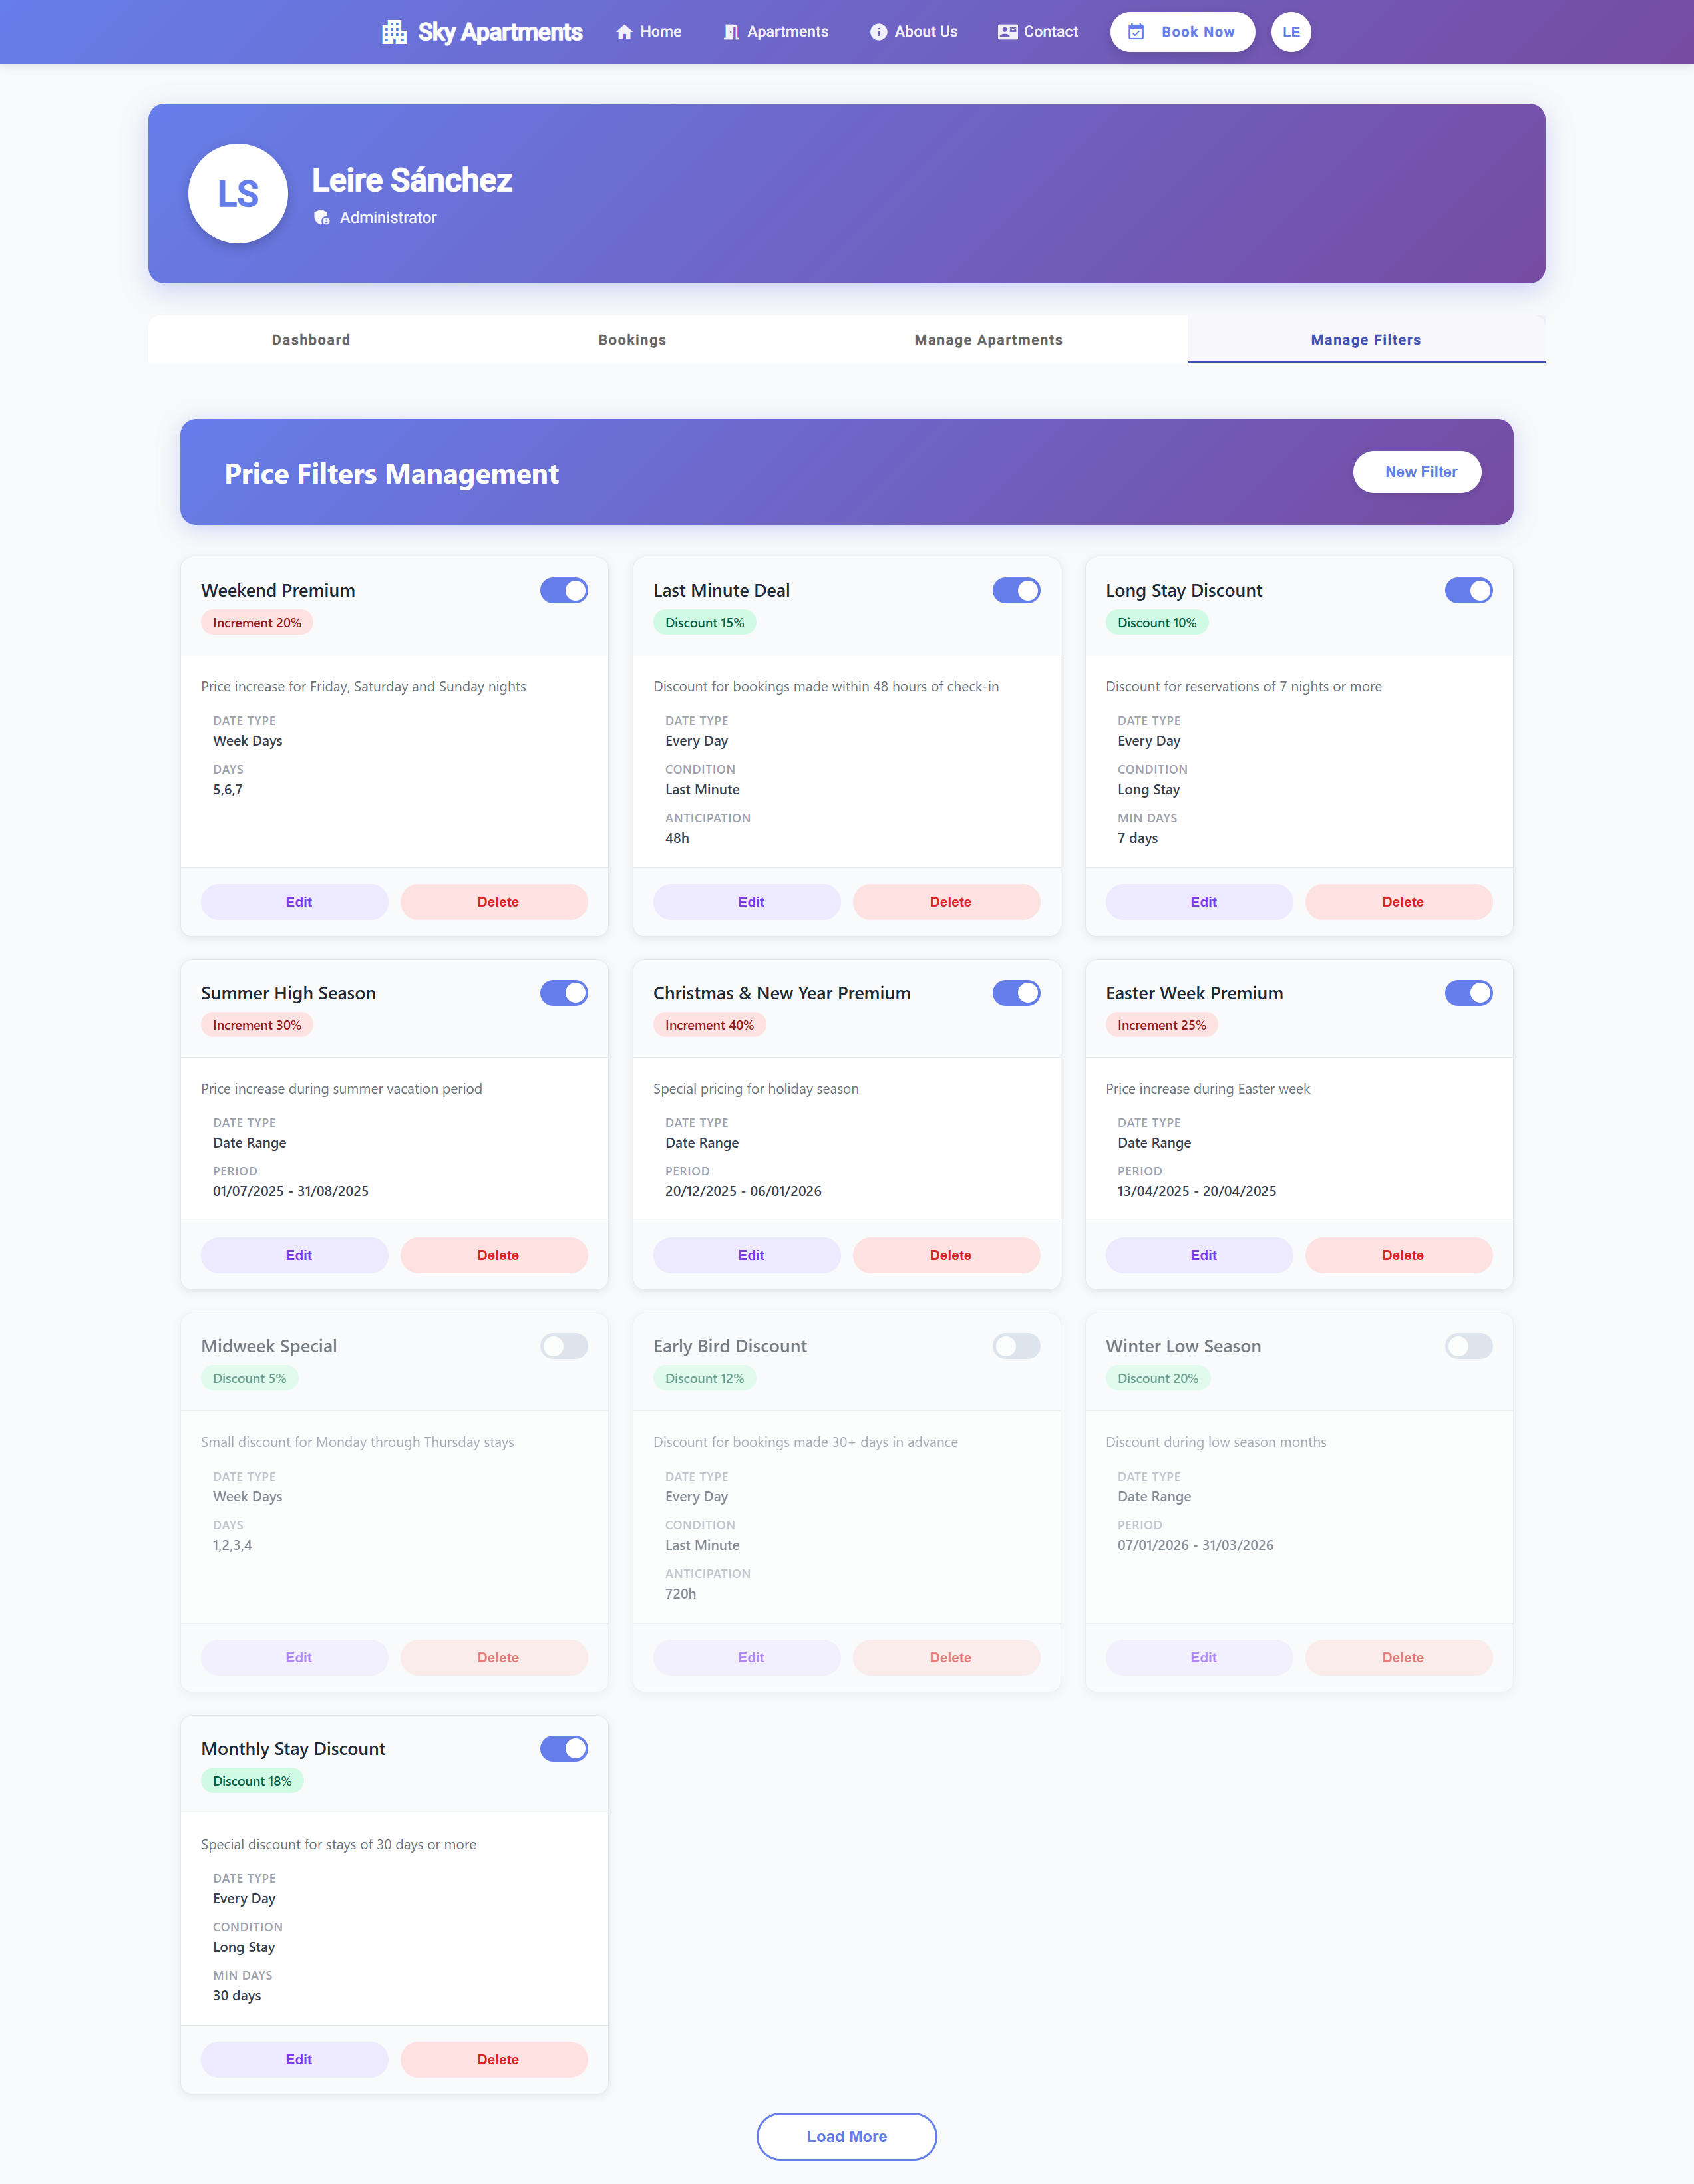
\includegraphics[width=0.9\textwidth]{img/admin_filters_v1.png}
    \caption{Interfaz de gestión y edición de filtros dinámicos de precios.}
    \label{fig:admin_filters}
\end{figure}

\subsection{Administración de Reservas}
Proporciona una vista en forma de lista paginada o calendario de todas las reservas del sistema. Incluye filtros avanzados para buscar reservas por estado, rango de fechas o nombre del apartamento, permitiendo una gestión operativa y eficiente incluso con grandes volúmenes de datos (ver Figura \ref{fig:admin_bookings}).

\begin{figure}[H]
    \centering
    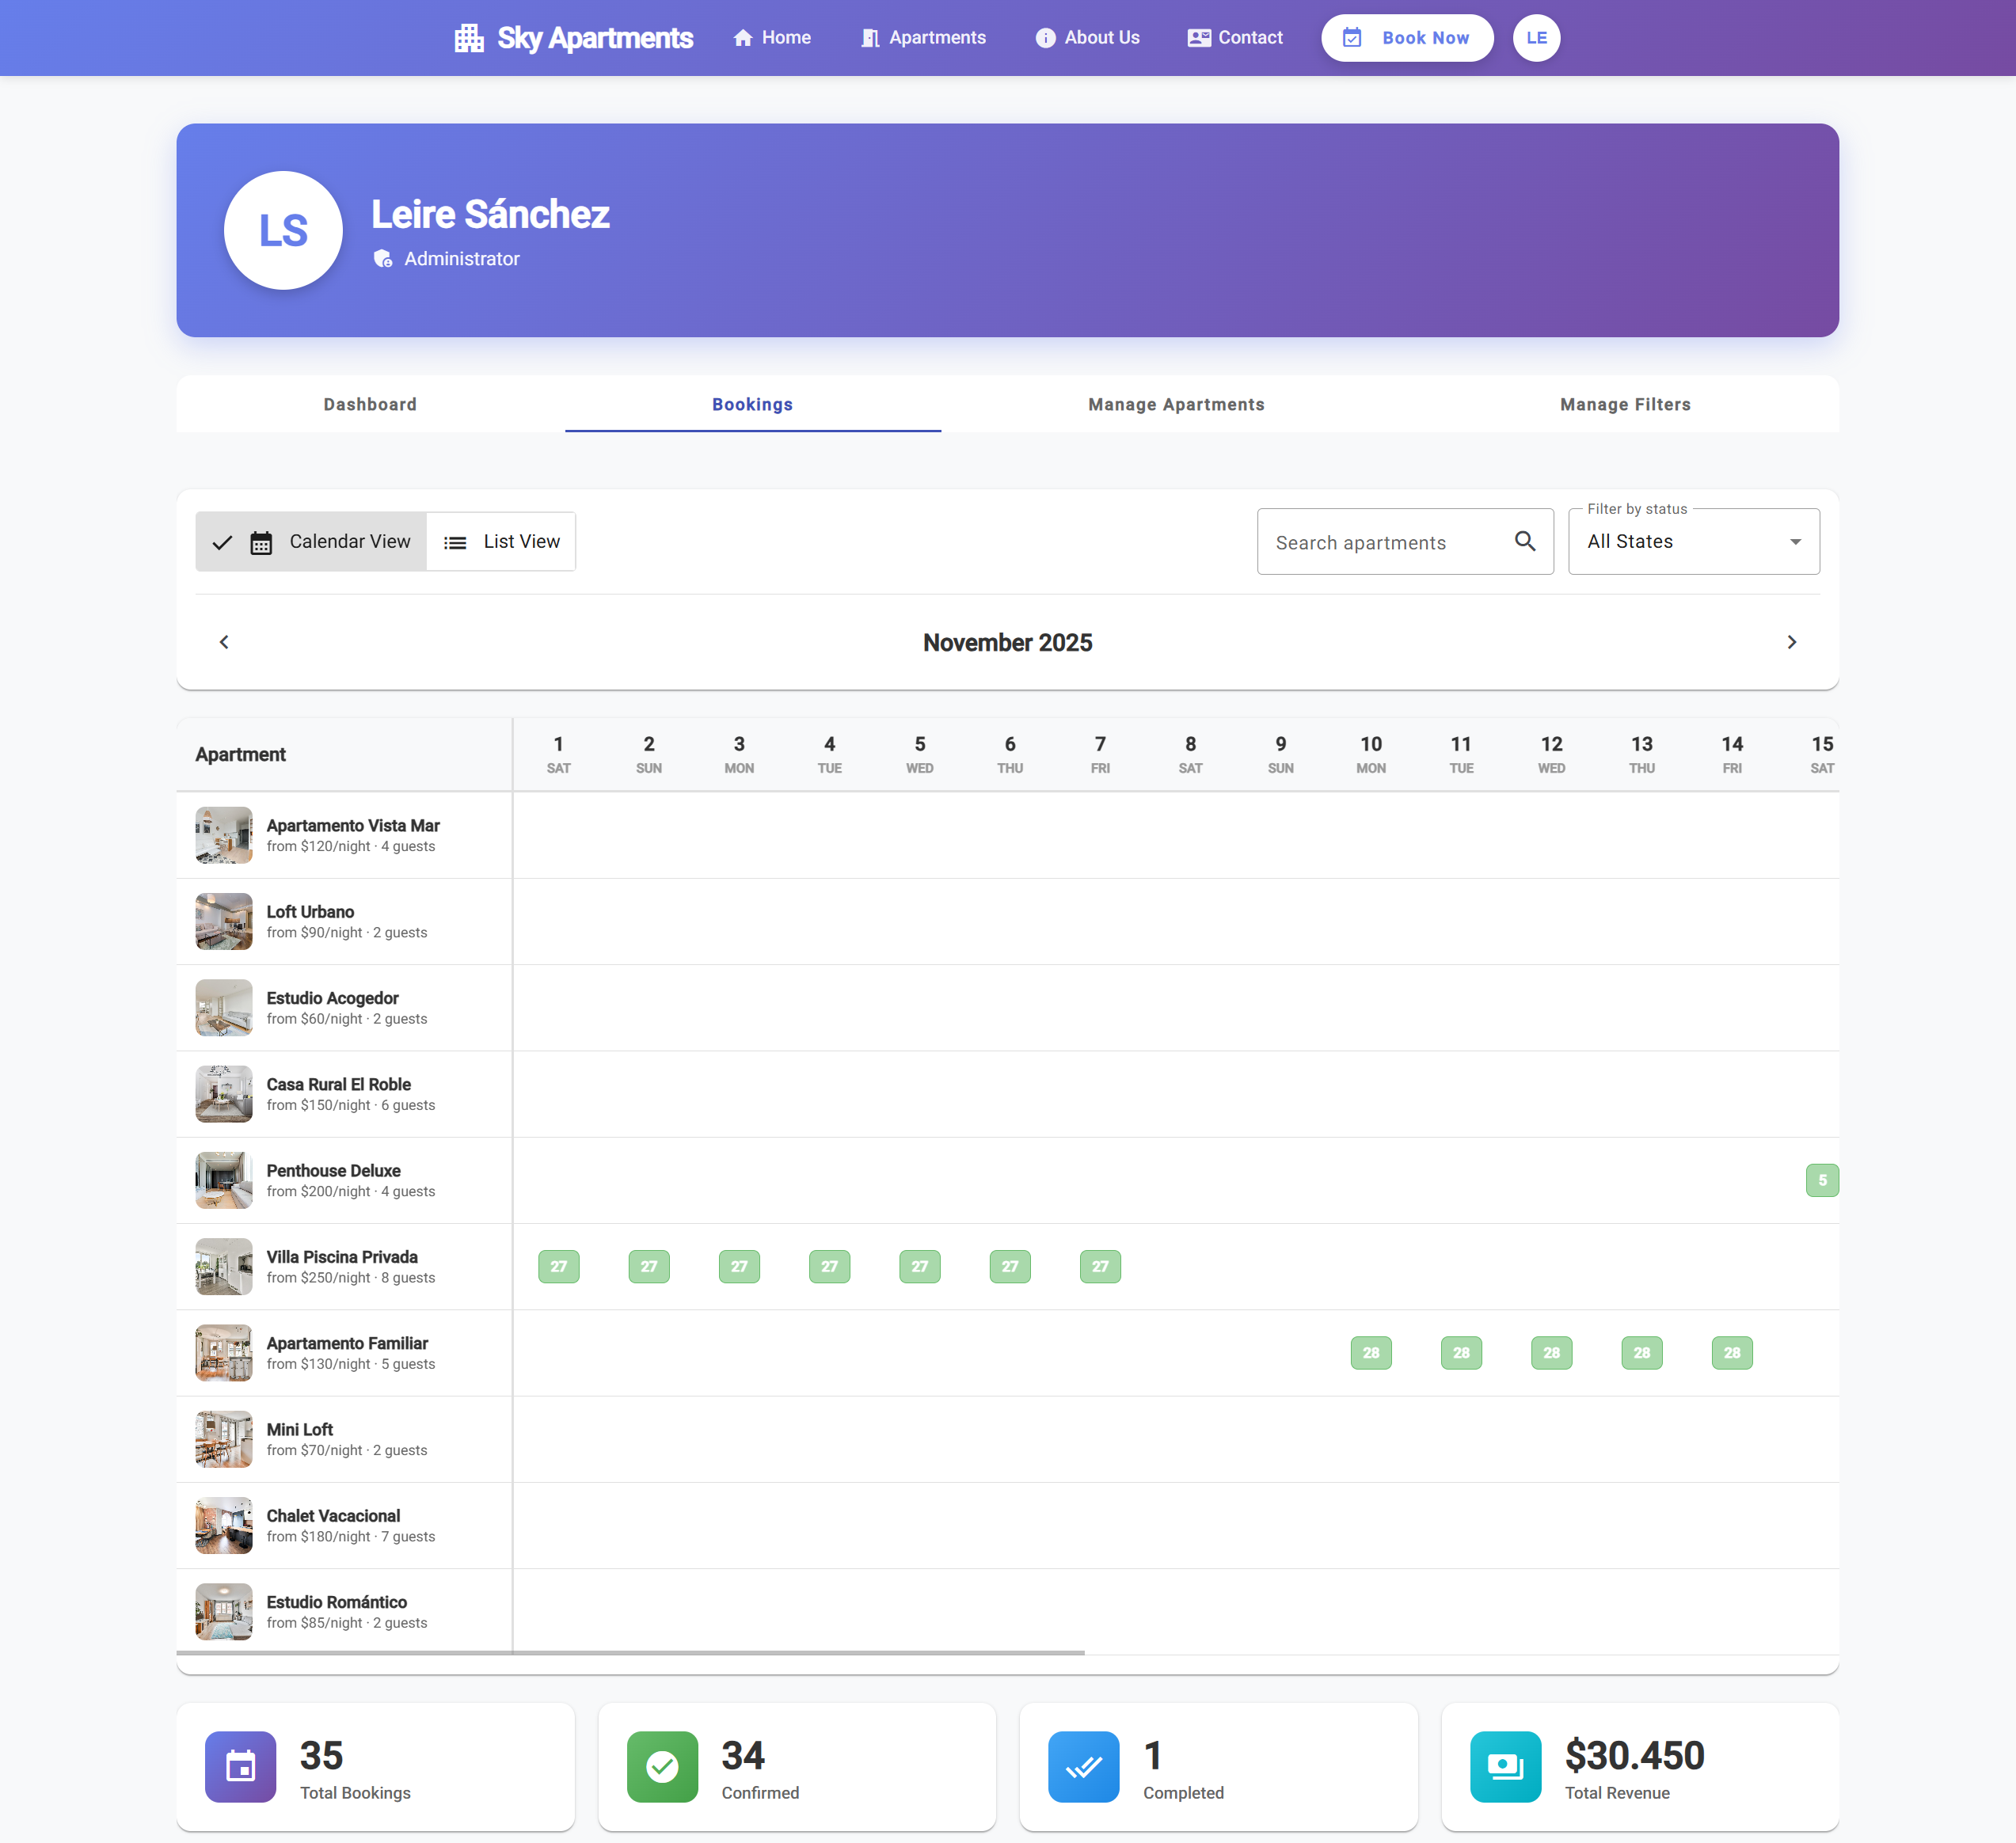
\includegraphics[width=0.9\textwidth]{img/admin_bookings_v1.png}
    \caption{Panel de control para la gestión y seguimiento de todas las reservas.}
    \label{fig:admin_bookings}
\end{figure}
